%%
%% This is file `sample-authordraft.tex', generated with the docstrip utility.
%%
%% The original source files were:
%%
%% samples.dtx  (with options: `authordraft')
%% 
%% IMPORTANT NOTICE:
%% 
%% For the copyright see the source file.
%% 
%% Any modified versions of this file must be renamed with new filenames distinct from sample-authordraft.tex.
%% 
%% For distribution of the original source see the terms for copying and modification in the file samples.dtx.
%% 
%% This generated file may be distributed as long as the original source files, as listed above, are part of the same distribution.
%% (The sources need not necessarily be in the same archive or directory.)
%%
%% The first command in your LaTeX source must be the \documentclass command.
%%

\documentclass[sigconf]{acmart}

%%
%% NOTE that a single column version may be required for submission and peer review.
%% This can be done by changing the \doucmentclass[...]{acmart} in this template to \documentclass[manuscript,screen,review]{acmart}
%% 
%% To ensure 100% compatibility, please check the white list of approved LaTeX packages to be used with the Master Article Template at
%% https://www.acm.org/publications/taps/whitelist-of-latex-packages 
%% before creating your document.
%% The white list page provides  information on how to submit additional LaTeX packages for review and adoption.
%% Fonts used in the template cannot be substituted; margin adjustments are not allowed.
%%

%%
%% START: My Packages
%%
\usepackage{caption}
\usepackage{subcaption}
\usepackage{algpseudocode}
\usepackage{algorithm}
\usepackage{tikz}
\usetikzlibrary{shapes, arrows, arrows.meta}
\newtheorem{lemma}{Lemma}
\usepackage{url}
\hyphenation{}
%% For algorithms...
\algnewcommand\algorithmicforeach{\textbf{for each}}
\algdef{S}[FOR]{ForEach}[1]{\algorithmicforeach\ #1\ \algorithmicdo}
\algnewcommand\algorithmicswitch{\textbf{switch}}
\algnewcommand\algorithmiccase{\textbf{case}}
\algdef{SE}[SWITCH]{Switch}{EndSwitch}[1]{\algorithmicswitch\ #1\ \algorithmicdo}{\algorithmicend\ \algorithmicswitch}
\algdef{SE}[CASE]{Case}{EndCase}[1]{\algorithmiccase\ #1}{\algorithmicend\ \algorithmiccase}
\algtext*{EndSwitch}
\algtext*{EndCase}
%%
%% END: My Packages
%%

\begin{document}

%%
%% The "title" command has an optional parameter, allowing the author to define a "short title" to be used in page headers.
%%
\title{Scalable Overlay Operations over DCEL Polygon Layers}
%\title[Scalable Implementation of a DCEL to Support Overlay Operations]{Scalable Implementation of Double Connected Edge Lists to Support Binary Overlay Operations Between Very Large Polygon Layers}

%%
%% The "author" command and its associated commands are used to define the authors and their affiliations.
%% Of note is the shared affiliation of the first two authors, and the "authornote" and "authornotemark" commands used to denote shared contribution to the research.
%%
\author{Andres O. Calderon-Romero, Amr Magdy, Vassilis J. Tsotras}
%\authornote{All authors contributed equally to this research.}
\email{acald013@ucr.edu, amr@cs.ucr.edu, tsotras@cs.ucr.edu}
%\author{Amr Magdy}
%\email{amr@cs.ucr.edu}
%\author{Vassilis Tsotras}
%\email{tsotras@cs.ucr.edu}
\affiliation{
  \institution{University of California, Riverside}
  \streetaddress{900 University Ave.}
 % \city{Riverside}
%  \state{CA}
 % \country{USA}
  \postcode{92521}
}

%%
%% By default, the full list of authors will be used in the page headers.
%% Often, this list is too long, and will overlap other information printed in the page headers.
%% This command allows the author to define a more concise list of authors' names for this purpose.
%%

\renewcommand{\shortauthors}{Calderon, et al.}

%%
%% The abstract is a short summary of the work to be presented in the article.
%%
\begin{abstract}
    TBD
\end{abstract}

%%
%% The code below is generated by the tool at http://dl.acm.org/ccs.cfm. Please copy and paste the code instead of the example below.
%%
\begin{CCSXML}
<ccs2012>
   <concept>
       <concept_id>10010147.10010169.10010170</concept_id>
       <concept_desc>Computing methodologies~Parallel algorithms</concept_desc>
       <concept_significance>500</concept_significance>
       </concept>
   <concept>
       <concept_id>10002951.10002952.10002971</concept_id>
       <concept_desc>Information systems~Data structures</concept_desc>
       <concept_significance>500</concept_significance>
       </concept>
   <concept>
       <concept_id>10010147.10010919.10010172.10003817</concept_id>
       <concept_desc>Computing methodologies~MapReduce algorithms</concept_desc>
       <concept_significance>500</concept_significance>
       </concept>
 </ccs2012>
\end{CCSXML}

\ccsdesc[500]{Computing methodologies~Parallel algorithms}
\ccsdesc[500]{Information systems~Data structures}
\ccsdesc[500]{Computing methodologies~MapReduce algorithms}

%%
%% Keywords. The author(s) should pick words that accurately describe the work being presented. Separate the keywords with commas.
%%
\keywords{spatial data structures, , computational geometry, overlay operators}

%%
%% This command processes the author and affiliation and title information and builds the first part of the formatted document.
%%
\maketitle

\section{Introduction}
The use of spatial data structures is ubiquitous in many spatial applications, ranging from spatial databases to computational geometry, robotics and geographic information systems \cite{samet-book}. 
%It has important advantages to offer to current spatial algorithms in particular the application of spatial indexes and opportunities to exploit proximity among the data.  
Spatial data structures have been used to improve the efficiency of various spatial queries, such as spatial joins, nearest neighbors, voronoi diagrams and robot motion planning.
Examples include grids \cite{gridfile}, R-trees \cite{rtree, rstar}, quadtrees \cite{quadtree}, etc.
%are widely reported in literature, other structures have been less the focus of attention.  In particular, 
There are also \textit{edge-list}  structures that have been typically utilized in applications as topological computations in computational geometry \cite{berg_computational_2008}.
%but their employment have been limited to very specific domains.  The use of such kind of structures has been reported in applications 
%like obtaining silhouettes of polyhedra, efficient Minkowksi sums, offset of polygons and diverse types of triangulations \cite{berg_computational_2008}.
%mainly in computational geometry projects.

The most commonly used data structure in the edge-list family is the Doubly Connected Edge List (DCEL).  A DCEL \cite{muller_finding_1978, preparata_computational_1985} is a data structure which collects topological information for the edges, vertices and faces contained by a surface in the plane. The DCEL and its components represent a planar subdivision of that surface. In a DCEL, the faces (polygons) represent the cells of the subdivision; the edges are boundaries which divide adjacent faces; and the vertices are the point endings between adjacent edges.
In addition to geometric and topological information a DCEL can be enhanced to provide further information.  For instance, a DCEL storing a thematic map for vegetation can store also information about the type and height the trees around the area \cite{berg_computational_2008}. 

The DCEL data structure has been used in various applications. For instance, the use of connected edge lists is cardinal to support polygon triangulations and their applications in surveillance (the Art Gallery Problem \cite{chvatal_combinatorial_1975, orourke_art_1987}) and robot motion planning (Minkowski sums \cite{berg_computational_2008, chew_convex_1993}).  DCELs are also used to perform polygon unions (for example, on printed circuit boards to support the simplification of connected components in an efficient manner \cite{fogel_cgal_2012}) as well as the computation of silhouettes from polyhedra \cite{fogel_cgal_2012, berberich_arrangements_2010} (applied frequently in computer vision and 3D graphics modelling \cite{boguslawski_modelling_2011}).

Edge-list data structures have also been utilized for the creation of thematic \textit{overlay maps}. In this problem, the input contains the DCELs of two polygon layers each capturing geospatial information and attribute data for different phenomena and the output is the DCEL of an overlay structure that combines the two layers into one. In many application areas such as ecology, economics and climate change, it is important to be able of join the input layers and match their attributes in order to unveil patterns or anomalies in data which can be highly impacted by location. Several operations can then be easily computed given an overlay; for instance, the user may want to find the \textit{intersection} between the input layers, identify their \textit{difference} (or symmetric difference), or create their \textit{union}. 

Spatial databases have been using spatial indexes (R-tree \cite{rtree, rstar}) to store and query polygons. Such methods use the \textit{filter and refine} approach where a complex polygon is abstracted by its Minimum Bounding Rectangle (MBR) that is inserted in the R-tree index. Finding the intersection between two polygon layers each indexed by a separate R-tree is then reduced to finding the pairs of MBRs from the two indexes that intersect (filter part). This is followed by the refine part, which, given two MBRs that intersect needs to compute the actual intersections between all the polygons these two MBRs contain. While MBR intersection is simple, computing the intersection between a pair of complex real-life polygons is a rather expensive operation (a typical 2020 US census track is a polygon with hundreds of edges). 

Moreover, using DCELs for overlay operations offers the additional advantage that the result is also a DCEL which can then be directly used for subsequent operations. For example, one may want to create an overlay between the intersection of two layers with another layer and so on. 

%\textcolor{red}{clarify paragraph} Furthermore, most of distributed techniques that have been used in this matter are oriented to a specific spatial operation (intersection, union or difference) and they have to be run from scratch if other operation is required.  In addition, current parallel techniques divide the data into partitions and replicate features if needed in order to solve the problem locally.  It could potentially increase the size of the problem.  

Even though the DCEL has important advantages for implementing overlay operations, current approaches are sequential in nature. This is problematic considering layers with thousands of polygons. For example, layers representing the 2020 US census tracks contains around 72K polygons; the execution time for computing the overlay over such files becomes prohibitive, taking days to get the results on a stock laptop. To the best of our knowledge there is no scalable solution to compute overlays over DCEL layers.

%Even sequential DCEL implementation are not new, nowadays, with the scale and volume of available geodata, the rise of big (spatial) data makes necessary to count with fast and efficient techniques for spatial analysis.  For example, today GIS researchers have to deal with spatial operations between layers collecting thousand of counties boundaries at nation-wide level.  The versatility and efficiency of the spatial methods is cardinal for their studies. Given the advantages shown by the DCEL data structure, it should be interesting to count with intermediate data structures that not just exploit the advantages of distributed frameworks but also allow multiple map overlay queries at the same time. 

%In addition, we already know that current topological data structures are common in computational geometry.  However, most implementations are sequential and they do not scale appropriately on large spatial datasets.  Moreover, distribute alternatives like parallel spatial joins add complexity due to spatial partitioning and replication and they are unable to run more than one operation once they have been created.

In this paper we describe the design and implementation of a scalable and distributed approach to compute the overlay between two DCEL layers. We first present a partition strategy that guarantees that each partition collects the required data from each layer DCEL to work independently, thus minimizing duplication and transmission costs over 2D polygons.  In addition, we present a merging procedure that collects all partition results and consolidates them in the final combined DCEL.  
%In section \ref{sec:strategy} we present and discuss the implementation of a novel strategy to divide the input data and build a distribute and scalable DCEL to be used 
Our approach has been implemented in a parallel framework (i.e., Apache Spark). 

Implementing a distributed overlay DCEL creates novel problems. First, there are potential challenges which are not present in the sequential DCEL execution. For example, the implementation should consider features such as \textit{holes} and \textit{multi-polygons} which could lay on different partitions.  Such features need to be connected with their components residing in other partitions so as to not compromise the correctness of the combined DCEL.  %Appropriate mechanism should be applied to solve these possible cases.

Secondly, once a distributed overlay DCEL has been built, it must support a set of binary overlay operations (namely \textit{union, intersection, difference} and \textit{symmetric difference}) in a transparent manner.  That is, such operators should take advantage of the scalability of the overlay DCEL and be able to run also in a parallel fashion.  Additionally, users should be able to apply the various operators multiple times without the need of rebuild the DCEL data structure.  %That means, that the binary operators should be applied on top of the distributed DCEL in a parallel fashion and , once it is done, the local results should be integrated together in order to remove any duplication and merging partial results obtained on contiguous partitions.

The rest of this paper is organized as follows. Section \ref{sec:related} presents related work while Section \ref{sec:prelim} discusses the basics of DCEL and the sequential algorithm.
In Section \ref{sec:methods} we present a partitioning scheme that enables parallel implementation of the overlay computation among DCEL layers; we also discuss the challenges presented in the DCEL computations by distributing the data and how to solve them efficiently. 
Two important optimizations are introduced in Section \ref{sec:alternative_methods}.
An extensive experimental evaluation appears in Section \ref{sec:experiments}, while Section \ref{sec:conclusions} concludes the paper.
%could arise.  We integrate a solution to solve cases such as isolated holes or empty partitions which could lost reference data during the distribution. We present an algorithm to detect and track partitions with orphans components and systematically search their neighborhood for related features.  

%Section \ref{sec:overlay} provides the details of the implementation of the binary overlay operators which query the DCEL.  The operations for intersection ($A \cap B$), union ($A \cup B$),  difference ($A - B$) and symmetric difference ($A \triangle B$) are available.  They are executed locally at each partition of the DCEL and then collecting and merging the results to provide the final answer.  The parallel execution take advantage of the distribution and efficiently exploits the locality to present the results.

%At the best of our knowledge, there is not a distributed and scalable DCEL implementation available that meet those criteria.  We think it could be a great tool to support key challenges and operations in Geoscience today.
\section{Related Work}
\label{sec:related}
The fundamentals of the DCEL are explained in the seminal paper \cite{muller_finding_1978} and \cite{preparata_computational_1985}.  Authors highlight among the main advantages of DCELs the opportunity of capturing topological information and allowing multiple overlay operations once the DCEL is created.  

An important reference for DCEL description and design should be \cite{berg_computational_2008}.  It states a DCEL can be constructed in $\mathcal{O}(n log(n))$ time using $\mathcal{O}(n)$ additional memory where $n$ is the number of vertices in the input layer \cite{freiseisen_colored_1998}. Once created, the DCEL allows binary overlay operations in $\mathcal{O}(n)$ time using $\mathcal{O}(n)$ additional space. 

Nowadays, sequential implementations of DCEL have been presented and used in diverse applications \cite{barequet_dcel_1998, boltcheva_topological-based_2020, freiseisen_colored_1998}. Although there is not reference to distributed DCEL implementations, other dynamic parallel data structures has been described \cite{challa_dd-rtree_2016, sabek_spatial_2017, li_scalable_2019}.  However, spatial indexes and spatial joins could support overlay operations in certain way but just for an individual operator at a time. 

Another works present parallel map overlay algorithms whose focus on GPU and multi-core architecture \cite{franklin_data_2018, magalhaes_fast_2015, puri_efficient_2013, puri_mapreduce_2013}.  Most of them use scan lines to partition the set of edges and hierarchical tree structures (octree or rtree) to partition the input data. However, as previous works, they test the implementation only with the intersection overlay operation. Even though, these works focus on solutions aim to multi-core architectures or GPGPU models which scalability can be affected by very large datasets.  In addition, implementations over the traditional multi-core ecosystem could not take total advantage of modern distributed memory frameworks such as Apache Spark.

Currently, few sequential implementations are available in the market.  Most important are LEDA\footnote{\url{https://www.algorithmic-solutions.com/}} \cite{mehlhorn_leda_1995}, Holmes3D\footnote{\url{http://www.holmes3d.net/graphics/}} \cite{holmes_dcel_2021} and CGAL\footnote{\url{https://www.cgal.org/}} \cite{fogel_cgal_2012}.  LEDA and Holmes3D are close-source software and limited access.  On the other hand, CGAL is an open-source project with a large trajectory in the area of computational geometry offering a wide-ranging number of packages and modules to support diverse areas offering a solid support for DCEL construction.

\section{Preliminaries}
\label{sec:prelim}

The DCEL \cite{muller_finding_1978} structure is used to represent an embedding of a planar subdivision in the plane. It provides efficient manipulation of the geometric and topological features of spatial objects (polygons, lines and points) using \textit{faces}, \textit{edges} and \textit{vertices} respectively.  
%It is used in many algorithms of computational geometry to handle polygonal subdivisions of the plane,for example to handle and store Voronoi diagrams and thematic maps.  It was originally proposed by \cite{muller_finding_1978} to handle convex polyhedra.
A DCEL uses three tables (relations) to store records for the faces, edges and vertices, respectively. 
An important characteristic is that all these records are defined using edges as the main component (thus termed as an edge-based structure). 
Examples appear in Tables \ref{tab:vertices}-\ref{tab:hedges} below, following the subdivision depicted in Figure \ref{fig:pre_dcel}.
%that contains records for each face, edge and vertex.  
%In addition to geometric and topological information it may also provides further data known as attribute information.  For instance, a DCEL storing a thematic map for vegetation can store also information about the type and height the trees around the area \cite{berg_computational_2008}.  
%The main advantage that a DCEL provides is the traversing of the faces of the planar subdivision visiting the edges around a vertex.

% Describe the inputs for the creation of a DCEL.  In our case it can be a set of polygons in a text format where each line describe the set of sorted vertices of each polygon or a saved DCEL which reads the three relations for faces, edges and vertices.

An edge corresponds to a straight line segment, shared by two adjacent faces (polygons). 
Each of these two faces will use this edge in its description; to distinguish, each edge has two \textit{half-edges}, one for each orientation (direction).
It is important to note that half-edges are oriented counter clockwise inside each face (Figure \ref{fig:pre_dcel}).
A half-edge is thus defined by its two vertices, one called the \textit{origin} vertex and the other the \textit{target} vertex, clearly specifying the half-edge's orientation (origin to target).
Each half-edge record contains references to its origin vertex, its face, its \textit{twin} half-edge, as well as the next and previous half-edges (using the orientation of its face); see Table \ref{tab:hedges}. These references are used as keys to the tables that contain the referred attributes. 

Figure \ref{fig:pre_dcel} shows half-edge $\overrightarrow{fe}$, its \textit{twin($\overrightarrow{fe}$)} (which is half-edge $\overrightarrow{ef}$), the \textit{next($\overrightarrow{fe}$)} (i.e. half-edge $\overrightarrow{ec}$) and the \textit{prev($\overrightarrow{fe}$)} (half-edge $\overrightarrow{df}$). Note the counter clockwise direction used by the half-edges comprising face $f_2$. 
The \textit{incidentFace} of a half-edge corresponds to the face that this edge belongs to (for example \textit{incidentFace}($\overrightarrow{fe}$) is face $f_2$).

Each vertex corresponds to a record in the vertex table (see Table \ref{tab:vertices}) that contains its coordinates as well as one of its incident half-edges. An incident half-edge is one whose target is this vertex. Any of the incident edges can be used; the rest of a vertex's incident half-edges can be found easily following next and twin half-edges.

Finally, each record in the faces table contains one of the face's half edges to describe the polygon's outer boundary (following this face's orientation); see Table \ref{tab:faces}. 
All other half-edges for this face's boundary can be easily retrieved following next half-edges in orientation order.
In addition to regular faces, there is one face that covers the area outside all faces; it is called the  \textit{unbounded} face (face $f_3$ in Figure \ref{fig:pre_dcel}). 
Since $f_3$ has no boundary, its boundary edge is set to \textit{nil} in Table \ref{tab:faces}.
Note, that polygons can contain one or more \textit{holes} (a hole is an area inside the polygon that does not belong to it). 
Each such hole is itself described by one of its half-edges; this information is stored in a list attribute (hole list) in the faces table. Note that in Table \ref{tab:faces} this list is empty as there are no holes in any of the faces in the example of Figure \ref{fig:pre_dcel}. 

%For the unbounded face their pointers are \textit{nil} in order to .

%In order to build a DCEL it begins with a set of edges, pair of two vertices, start and end, which define its orientation (direction). We assume every edge is an straight line segment. A face is a polygonal region whose boundary is formed by connected subset of edges that does not contain any additional point on a previous edge or a vertex.  The main idea is that the faces of the resulting DCEL can be able to reconstruct the original polygons \cite{berg_computational_2008}.

%Particularly, a DCEL stores their main components in a set of records using a half-edge structure.  For convenience, since an edge divides contiguous faces, each edge is replaced by two half-edges to link each face.  


\begin{figure}
    \centering
    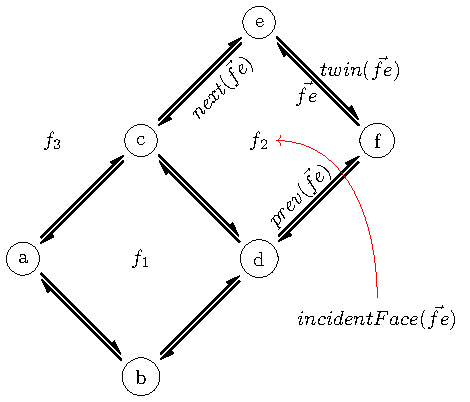
\includegraphics[width=0.9\linewidth]{figures/dcel_example/dcel_example}    
    \caption{Components of the DCEL structure.}\label{fig:pre_dcel}
    \Description[Components of the DCEL structure]{This figure shows the components of a DCEL.}
\end{figure}

%The doubly-connected edge list consists of three collections of records: one for the vertices, one for the faces, and one for the half-edges.  These records store the following geometric and topological information:

%The vertex record of a vertex $v$ stores the coordinates of $v$ in a field called $coordinates(v)$. It also stores a pointer incidentEdge $(v)$ to an arbitrary half-edge that has $v$ as its origin (see table \ref{tab:vertices}).

%The face record of a face $f$ stores a pointer outerComponent $(f)$ to some half-edge on its outer boundary. For the unbounded face this pointer is \textit{nil}. It also stores a list innerComponents $(f)$, which contains for each hole in the face a pointer to some half-edge on the boundary of the hole (see table \ref{tab:faces}).

%The half-edge record of a half-edge $\overrightarrow{e}$ stores a pointer to its origin, a pointer $twin(\overrightarrow{e}$) to its twin half-edge, and a pointer incident Face$(\overrightarrow{e}$) to the face that it bounds. We don’t need to store the destination of an edge, because it is equal to $origin(twin(\overrightarrow{e}$)). The origin is chosen such that incidentFace $(\overrightarrow{e})$ lies to the left of $\overrightarrow{e}$ when it is traversed from origin to destination. The half-edge record also stores pointers $next(\overrightarrow{e}$) and $prev(\overrightarrow{e})$ to the next and previous edge on the boundary of incidentFace $(\overrightarrow{e})$. Thus $next(\overrightarrow{e}$) is the unique half-edge on the boundary of incidentFace $(\overrightarrow{e}$) that has the destination of $\overrightarrow{e}$ as its origin, and $prev(\overrightarrow{e}$) is the unique half-edge on the boundary of incidentFace $(\overrightarrow{e}$) that has $origin(\overrightarrow{e}$) as its destination (see table \ref{tab:hedges}).

\begin{table*} \label{tab:records}
\begin{minipage}{0.3\textwidth}
    \centering
    \begin{tabular}{c c c}
        \toprule
        vertex & coordinates & incident edge \\
        \midrule
        a      & (0,2)  & $\vec{ba}$ \\
        b      & (2,0)  & $\vec{db}$ \\
        c      & (2,4)  & $\vec{dc}$ \\
        \vdots & \vdots & \vdots     \\
        \bottomrule
    \end{tabular}
    \caption{Vertex records.}\label{tab:vertices}
\end{minipage}\hfill % maximize the horizontal separation
\begin{minipage}{0.3\textwidth}
    \centering
    \begin{tabular}{c c c} 
        \toprule
             & boundary  & hole\\
        face & edge      & list\\
        \midrule
        $f_1$ & $\vec{ab}$ & $nil$ \\
        $f_2$ & $\vec{fe}$ & $nil$ \\
        $f_3$ & $nil$      & $nil$ \\
        \bottomrule
    \end{tabular}
    \caption{Face records.}\label{tab:faces}
\end{minipage}\hfill % maximize the horizontal separation
\begin{minipage}{0.4\textwidth}
    \centering
    \begin{tabular}{c c c c c c} 
        \toprule
        half-edge & origin & face & twin & next & prev \\
        \midrule
        $\vec{fe}$ & f & $f_2$  & $\vec{ef}$ & $\vec{ec}$ & $\vec{df}$ \\
        $\vec{ca}$ & c & $f_1$  & $\vec{ac}$ & $\vec{ab}$ & $\vec{dc}$ \\
        $\vec{db}$ & d & $f_3$  & $\vec{bd}$ & $\vec{ba}$ & $\vec{fd}$ \\
        \vdots     & \vdots & \vdots & \vdots     & \vdots     & \vdots     \\
        \bottomrule
    \end{tabular}
    \caption{Half-edge records.}\label{tab:hedges}
\end{minipage}
\end{table*}

An important advantage with the DCEL structure is that a user can combine two DCELs from different layers over the same area (e.g. the census tracks from two different years) and compute their \textit{overlay} which is a DCEL structure that combines the two layers into one. Other operators like the intersection, difference etc. can then be computed from the overlay very efficiently.
Given two DCEL layers $S_1$ and $S_2$, a face $f$ appears in their overlay  $O(S_1, S_2)$ if and only if there are faces $f_1$ in $S_1$ and $f_2$ in $S_2$ such that $f$ is a maximal connected subset of $f1 \cap f2$ \cite{berg_computational_2008}.  
This property implies that the overlay $O(S_1, S_2)$ can be constructed using the half-edges from $S_1$ and $S_2$ . 

The sequential algorithm \cite{fogel_cgal_2012} to construct the overlay between two DCELs first extracts the half-edge segments from the half-edge tables and then finds intersection points between half-edges from the two layers (using a sweep line approach) \cite{berg_computational_2008}. 
The intersection points found will become new vertices of the resulting overlay. 
If an existing half-edge contains an intersection point it is split into two new half-edges. 
Using the list of outgoing and incoming half-edges for the newly added vertices (intersection points) the algorithm can compute the attributes for the records of the new half-edges. For example, the list of outgoing and incoming half-edges at each new vertex will be used to update the next, previous and twin pointers. Finally, records for faces and vertices tables are also updated with the new information. 

\begin{figure}
    \centering
    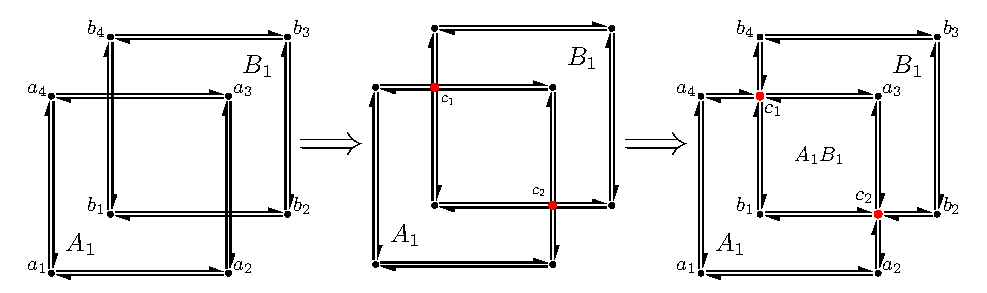
\includegraphics[width=\linewidth]{figures/dcel_seq/dcel2}
    \caption{Sequential computations of an overlay of two DCEL layers.}\label{fig:dcel_seq}
    \Description[Sequential computations of an overlay of two DCEL layers.]{This figure shows the sequential computations of an overlay of two DCEL layers..}
\end{figure}

Figure \ref{fig:dcel_seq} illustrates an example for computing the overlay between two DCEL layers with one face each ($A_1$ and $B_1$ respectively), that overlap over the same area. First, intersection points are found and create new vertices in the overlay (red vertices $c_1$ and $c_2$). Finally, new half edges are created around these new vertices. 
As a result, face $A_1$ is modified (to an L-shaped boundary) as does face $B_1$, while a new face $A_1B_1$ is created. 
Since this new face is the intersection of the boundaries of $A_1$ and $B_1$, it label contains the concatenation of both face labels. 
By convention \cite{berg_computational_2008}, even though $A_1$ changes its shape, it does not change its label since its new shape is created by its intersection with the unbounded face of $B_1$; similarly the new shape of $B_1$ maintains its original label. 

%To do that, these list is sorted clockwise around the vertex and traversed to identify pairs of half-edges.  If a pair of half-edges are the same but in opposite direction, the twin pointer will be updated between each other, otherwise the next and previous pointers will be updated accordingly. 

%Figure \ref{fig:part2} illustrates the procedure (still working on it...). Here we can see that the clockwise order around new vertex $e$ is $\{\overrightarrow{eb}$, $\overrightarrow{be}$, $\overrightarrow{ec}$, $\overrightarrow{ce}$, $\overrightarrow{ed}$, $\cdots\}$.  It is easy to see that the first pair of half-edges corresponds to opposite ones so the twin pointer will be updated between half-edges $\overrightarrow{eb}$ and $\overrightarrow{be}$. In contrast, for the following pair, next pointer of  $\overrightarrow{be}$ will be set as $\overrightarrow{ec}$ and conversely for the previous pointer.  The updating continues until completing all the pairs. 

%The main advantage of DCELs is the scalability and reuse of the structure for different operators. 

Once the overlay of two DCELs is computed, queries like their intersection, union, difference etc. (Figure \ref{fig:overlay_operations}) can be performed in linear time to the number of faces. 
Clearly, the overlay space requirement remains linear to the number of vertices, edges and faces.  
Since an overlay is itself a DCEL, it can support the traditional DCEL operations (e.g., find the boundary of a face, access a face from an adjacent one, visit all the edges around a vertex, etc.)

\begin{figure*}
    \centering
    \tikzset{    
    node1/.style={
        above right
    }
}
\scalebox{0.5}{
    \begin{tikzpicture}
        \node[node1,label={$A \cup B$}]           at (0,0)  {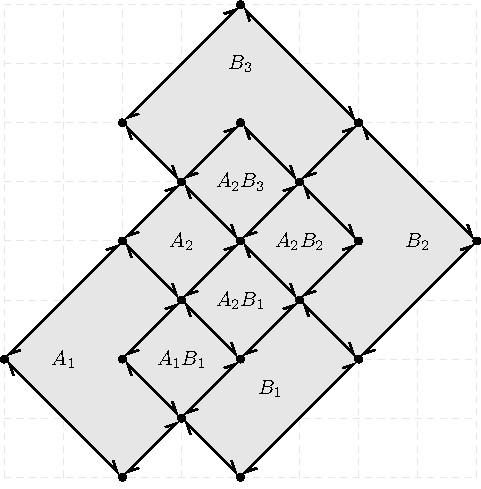
\includegraphics[scale=0.75]{figures/04/DCELUnion}};
        \node[node1,label={$A \cap B$}]           at (7,0)  {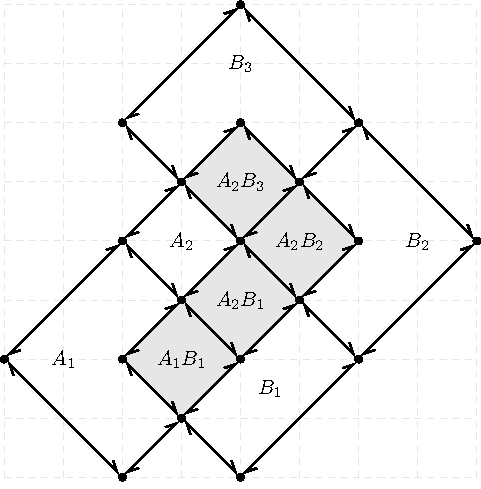
\includegraphics[scale=0.75]{figures/04/DCELIntersection}};
        \node[node1,label={$A \setminus B$}]      at (14,0) {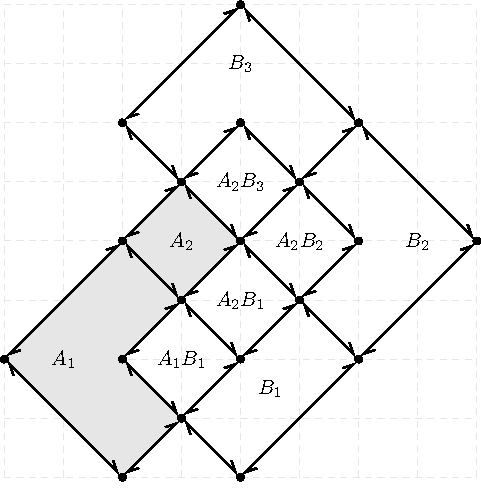
\includegraphics[scale=0.75]{figures/04/DCELDiffA}};
        \node[node1,label={$B \setminus A$}]      at (21,0) {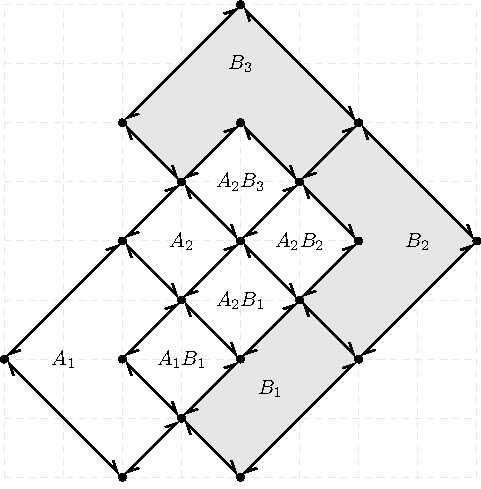
\includegraphics[scale=0.75]{figures/04/DCELDiffB}};
        \node[node1,label={$A \bigtriangleup B$}] at (28,0) {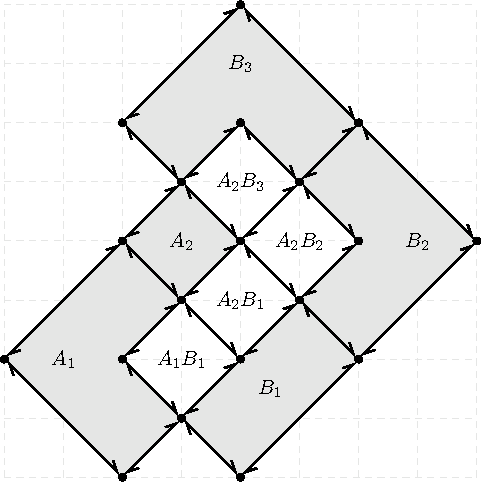
\includegraphics[scale=0.75]{figures/04/DCELDiff}};
    \end{tikzpicture}
}
    \caption{Examples of overlay operators supported by DCEL.}\label{fig:overlay_operations}
    \Description[Results of the overlay operations]{This figure shows the results of the overlay operations supported by the scalable DCEL.}
\end{figure*}

\section{Scalable Overlay Construction} \label{sec:methods}

The overlay computation depends on the size of the input DCELs and the size of the resulting overlay. The DCEL of a planar subdivision $S_1$ has size $O(n_1)$ where $n_1$ = $\Sigma (vertices_1 + edges_1 + faces_1$). 
%If complexity of $S_1$ is $n_1$ and complexity of $S_2$ is $n_2$, let $n = n_1 + n_2$.  So, 
The sequential algorithm constructing the overlay of $S_1$ and $S_2$ takes $O(n \log n + k \log n)$ time, where $n = n_1 + n_2$ and $k$ is the size of their overlay.
Note that $k$ depends on how many intersections occur between the input DCELs, which can be very large \cite{berg_computational_2008}. 
%It can be seen that inputs with a large number of edges will impact significantly the performance of the sequential algorithm.

While the sequential algorithm is efficient with small DCEL layers, it suffers when the input layers are large and have many intersections. 
For example, creating the overlay between the DCELs of two census tracks (from 2000 and 2010) from California (each with 7K-8K polygons and 2.7M-2.9M edges) took about 800sec on an Intel Xeon CPU at 1.70GHz (see Section \ref{sec:experiments}). 
With DCELs corresponding to the whole US, the algorithm crashed. 

Nevertheless, the overlay computation can take advantage of partitioning (and thus parallelism), by observing that the edges in a given area of one input layer, can only intersect with edges from the same area in the other input layer. 
One can thus spatially partition the two input DCELs using a spatial index (or grid) and then compute the overlay within each partition; such computations are independent and can be performed in parallel. 
While this is a high level view of our scalable approach, there are various challenges, including how to deal with edges that cross partitions, how to manage the extra complexity introduced by \textit{orphan} holes (i.e., when holes and their polygons are in different partitions), how and where to combine partition overlays into a global overlay, as well as how to balance the computation if one layer is much larger than the other. 
%The current challenge is the construction of a distributed and scalable DCEL structure that allows the querying of overlay operations, such as intersection and difference, over a large set of polygons.  The main idea of the solution is to partition the edges from each of the polygons using a spatial data structure (for instance, a quadtree).  Edges contained at each section of the partitioning will be the input of a local DCEL which will store the information of the vertices, half-edges and faces for their edges clipped to the boundary of its spatial partition.  Each local DCEL can be seen as an individual structure which can be queried and the solution will be later merged with the other local DCELs in their neighbourhood to complete the final answer. 



\subsection{Partition strategy} \label{sec:strategy}
The main idea of the partition strategy is to split the study area into no-overlapping cells which could be processed independently in a local basis.  
We could use a simple grid to divide the area but more suitable spatial indices, such as quadtrees, will help to assign a similar number of edges to each cell. 
The proposal can be summarized in the following steps: (i) Partition the input layers and build local DCEL representations of them at each cell; and (ii) Compute the overlay of the local DCELs locally scaling the processing cost. 
Overlay operators and other functions can be run over the local overlays and then be collected back to generate the final answer.  

The parallel approach is illustrated in figure \ref{fig:overlay_parted}.  First, we will use a sample of edges from both input layers to create cells which will spatially partition the space into disjoint areas.  
In the example, a simple grid is used but any spatial index can be applied (in our experiments we use quadtrees for better balance and edge distribution).
We will use those cells to clip the input layers to forced them to lie inside of the boundaries of a cell. 
If a face is split by the boundary of a cell, new edges (following the border) will be added to ensure the faces will be closed paths,
It ensures that all the needed edges for computation are available at each partition. 
Although it will increase the number of edges, we expect that the gain during parallel processing will make the addition worthwhile.

\begin{figure*}
    \centering
    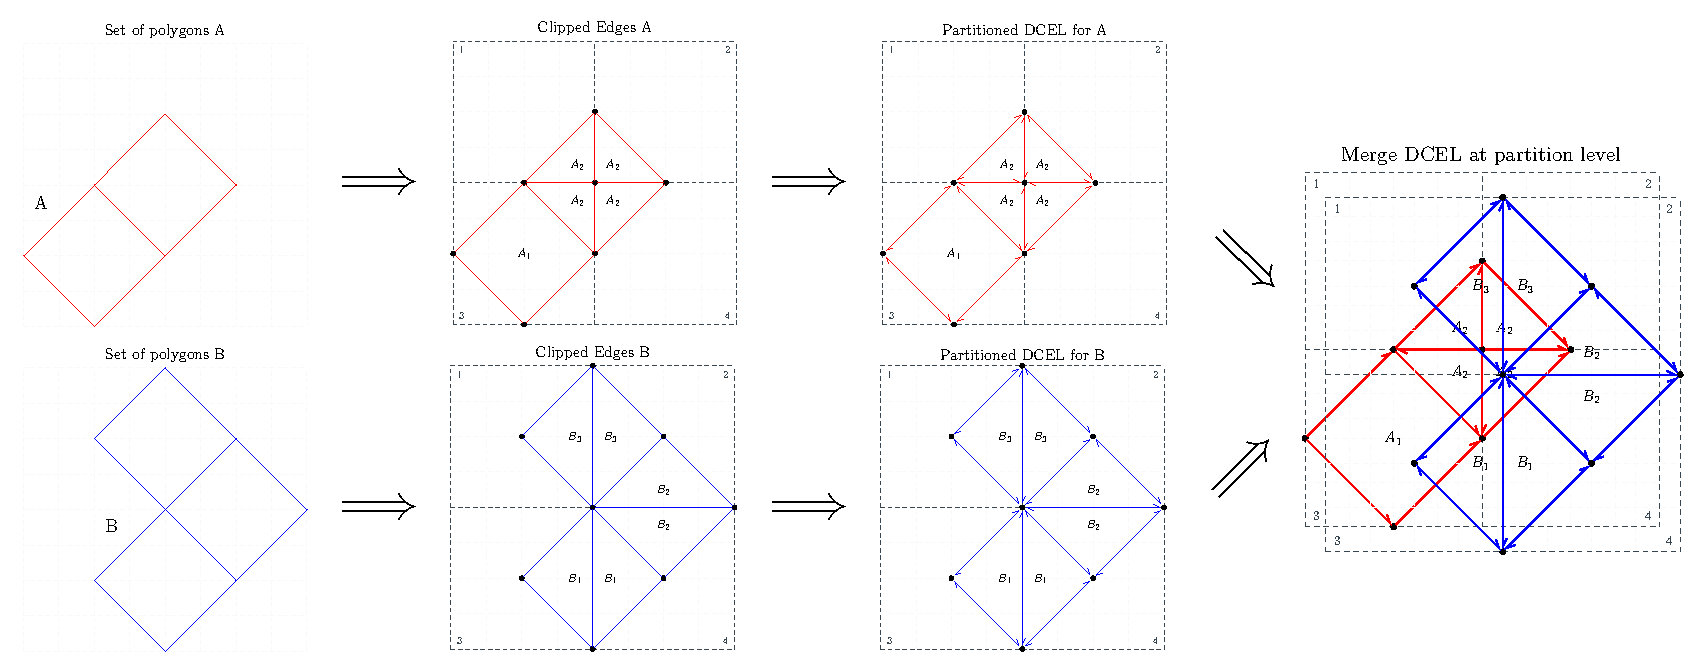
\includegraphics[width=\textwidth]{figures/01-OverlayParted}
    \caption{Partition scheme.}\label{fig:overlay_parted}
    \Description[Partition schema]{This figure illustrates the partition schema used to distribute the data.}
\end{figure*}

Now each cell have the enough data to build a DCEL representation of the input for each layer.  Data for each cell will be marked appropriately and submitted to different nodes to be processed in parallel.  
Note that the same partition schema (set and shape of cells) is used in both layers.  That is important due to it allows one-to-one matching between corresponding partitions in both layers.
Once the edges from the input have been distributed to the corresponding node, the sequential algorithm create a DCEL for each input and compute the corresponding overlay. 

Figure \ref{fig:part2} depicts an overview of the process taking as example the polygons and edges of partition 2 of figure \ref{fig:overlay_parted}.  Similarly, figure \ref{fig:merged_dcel} shows the overlay DCEL once all the partitions have been processed. 
Note that red half-edges have been introduced artificially by the partition strategy but they are marked accordingly to be removed after the collect back process.

\begin{figure}
    \centering
    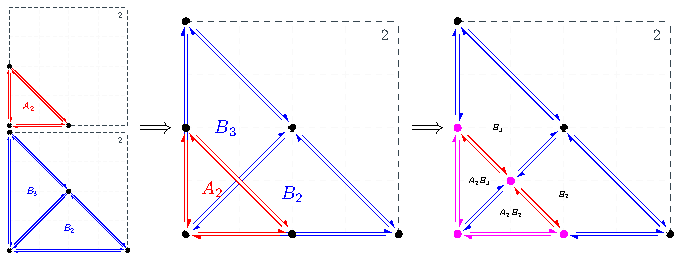
\includegraphics[width=0.9\linewidth]{figures/02-Part2}
    \caption{Overlay of local DCEL for partition 2.}\label{fig:part2}
    \Description[Overlay of local DCELs for a particular partition]{This figure shows how the local DCELs works in a particular example.}
\end{figure}

\begin{figure}
    \centering
    \tikzset{    
    barbarrow/.style={ % style that just defines the arrow tip
        %>={Straight Barb[left,length=5pt,width=5pt]},
        >={Triangle[left,length=5pt,width=5pt]},
        double,
        semithick,
        <->
    },
    whites/.style={
        thick, 
        color=white
    }
}
\definecolor{light-gray}{gray}{0.9}
\scalebox{0.75}{
\begin{tikzpicture}
    \tikzstyle{node1}=[draw,scale=0.4,shape=circle,color=black,fill=black]
    \tikzstyle{node2}=[draw,scale=0.4,shape=circle,color=red,fill=red]    
    \draw[color=light-gray, style=dashed] (0,0) grid (8,8);
    \draw[color=red, style=dashed, step=4] (0,0) grid (8,8);
    \node[node1] (A) at (0,2) {};    \node[node1] (C) at (2,0) {};
    \node[node1] (D) at (2,2) {};    \node[node1] (E) at (2,4) {};
    \node[node1] (F) at (2,6) {};    \node[node1] (G) at (3,1) {};
    \node[node1] (H) at (3,3) {};    \node[node1] (I) at (3,5) {};
    \node[node1] (J) at (4,0) {};    \node[node1] (K) at (4,2) {};
    \node[node1] (L) at (4,4) {};    \node[node1] (M) at (4,6) {};
    \node[node1] (N) at (4,8) {};    \node[node1] (O) at (5,3) {};
    \node[node1] (P) at (5,5) {};    \node[node1] (Q) at (6,2) {};
    \node[node1] (R) at (6,4) {};    \node[node1] (S) at (6,6) {};
    \node[node1] (T) at (8,4) {};

    \node at (1,2)      {$A_1$};
    \node at (6.5,4.6)  {$B_2$};
    \node at (6.5,3.4)  {$B_2$};
    \node at (3.4,6.5)  {$B_3$};
    \node at (4.6,6.5)  {$B_3$};
    \node at (4.6,1.5)  {$B_1$};
    \node at (3.6,1)    {$B_1$};
    \node at (3,4.4)    {$A_2$};
    \node at (3,3.6)    {$A_2$};
    \node at (3,2)              {$A_1B_1$};
    \node[scale=0.6] at (3.6,3) {$A_2B_1$};
    \node[scale=0.6] at (4.4,3) {$A_2B_1$};
    \node[scale=0.6] at (5,4.4) {$A_2B_2$};
    \node[scale=0.6] at (5,3.6) {$A_2B_2$};
    \node[scale=0.6] at (3.6,5) {$A_2B_3$};
    \node[scale=0.6] at (4.4,5) {$A_2B_3$};
    
    \draw[barbarrow] (A) -- (C);\draw[barbarrow] (A) -- (E);
    \draw[barbarrow] (C) -- (G);\draw[barbarrow] (D) -- (G);
    \draw[barbarrow] (D) -- (H);\draw[barbarrow] (E) -- (H);
    \draw[barbarrow] (E) -- (I);\draw[barbarrow] (F) -- (I);
    \draw[barbarrow] (F) -- (N);\draw[barbarrow] (G) -- (J);
    \draw[barbarrow] (H) -- (L);\draw[barbarrow] (I) -- (L);
    \draw[barbarrow] (I) -- (M);\draw[barbarrow] (J) -- (Q);
    \draw[barbarrow] (G) -- (K);\draw[barbarrow] (H) -- (K);
    \draw[barbarrow] (K) -- (O);\draw[barbarrow] (L) -- (O);
    \draw[barbarrow] (L) -- (P);\draw[barbarrow] (M) -- (P);
    \draw[barbarrow] (N) -- (S);\draw[barbarrow] (O) -- (Q);
    \draw[barbarrow] (O) -- (R);\draw[barbarrow] (P) -- (R);
    \draw[barbarrow] (P) -- (S);\draw[barbarrow] (Q) -- (T);
    \draw[barbarrow] (S) -- (T);
    
    \draw[whites] (A) -- (C);\draw[whites] (A) -- (E);
    \draw[whites] (C) -- (G);\draw[whites] (D) -- (G);
    \draw[whites] (D) -- (H);\draw[whites] (E) -- (H);
    \draw[whites] (E) -- (I);\draw[whites] (F) -- (I);
    \draw[whites] (F) -- (N);\draw[whites] (G) -- (J);
    \draw[whites] (H) -- (L);\draw[whites] (I) -- (L);
    \draw[whites] (I) -- (M);\draw[whites] (J) -- (Q);
    \draw[whites] (G) -- (K);\draw[whites] (H) -- (K);
    \draw[whites] (K) -- (O);\draw[whites] (L) -- (O);
    \draw[whites] (L) -- (P);\draw[whites] (M) -- (P);
    \draw[whites] (N) -- (S);\draw[whites] (O) -- (Q);
    \draw[whites] (O) -- (R);\draw[whites] (P) -- (R);
    \draw[whites] (P) -- (S);\draw[whites] (Q) -- (T);
    \draw[whites] (S) -- (T);
    
    \draw[barbarrow, color=red] (R) -- (T);\draw[whites] (R) -- (T);
    \draw[barbarrow, color=red] (M) -- (N);\draw[whites] (M) -- (N);
    \draw[barbarrow, color=red] (K) -- (J);\draw[whites] (K) -- (J);
    \draw[barbarrow, color=red] (L) -- (E);\draw[whites] (L) -- (E);
    \draw[barbarrow, color=red] (L) -- (R);\draw[whites] (L) -- (R);
    \draw[barbarrow, color=red] (L) -- (M);\draw[whites] (L) -- (M);
    \draw[barbarrow, color=red] (L) -- (K);\draw[whites] (L) -- (K);
\end{tikzpicture}
}    
    \caption{Result of the overlay DCEL.}\label{fig:merged_dcel}
    \Description[Result of the overlay DCEL]{This figure shows what would be the results of the overlay DCEL procedure.}
\end{figure}

At this point, we have access to a distributed spatial data structure which collects the individual DCEL representations (and its topological and geometric information) of the full study area at local basis.  It is easy to see that we can run overlay operators in parallel over the local DCELs and then just collect and merge the results to unify a final answer.  For example, figure \ref{fig:overlay_parted2} illustrates the process to query for the intersection results over the input polygons described in figure \ref{fig:overlay_parted}.  

\begin{figure}[!ht]
    \centering
    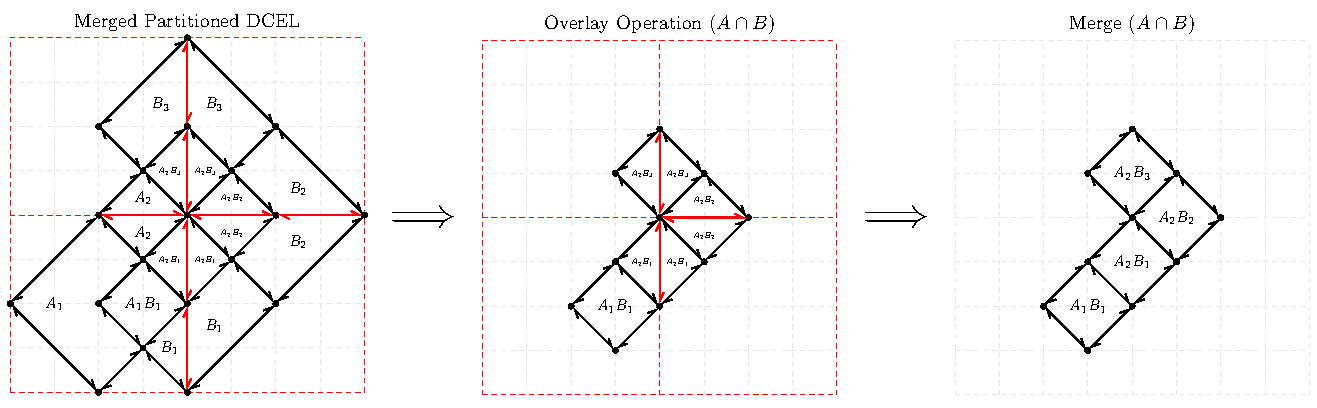
\includegraphics[width=\linewidth]{figures/03-OverlayParted2}
    \caption{Example of an overlay operation querying the distributed DCEL.} \label{fig:overlay_parted2}
    \Description[An example of an overlay operation]{This figure shows an example of an overlay operation querying the distributed DCEL.}
\end{figure}

The results of the overlay operators supported by the scalable DCEL are the same shown in figure \ref{fig:overlay_operations}.  To obtain the results the faces are filtered locally according to the characteristics of their label.  For intersection ($A \cap B$), it filters just faces where its label contains both letters (A and B); for symmetric difference ($A \bigtriangleup B$), it filters faces where its labels contains just one of the letters (A or B).  For the case of difference between the layers ($A \setminus B$ or $B \setminus A$), it filters faces and labels according to the requested letter (either A or B). In the case of union ($A \cup B$), all the faces are retrieved. 

\subsection{Parallel DCEL Computation}

During the partition process, the edges of each polygon are attached with pointers to their next and previous edge according to their order in the polygon's vertices.  As explained before, a spatial index is used to assign each edge to a particular cell.  Each edge is queried in the spatial data structure and it is labeled with the cell where it is contained.  If a edge covers multiples cell it is replicated in each one but clipped to the corresponding cell boundary.  In addition, edges representing the boundary of the cell are added to complement the edges enclosed in each cell.  Those artificial edges are marked accordingly to be removed during the merge stage.

The edges of the cell added at this stage are useful to complete the local DCEL.  It will allow that the resulting DCEL will enclose the full area of the cell and the local DCEL at each cell matches with the local DCEL of the other layer during the merge process.  The half-edges which intersect the boundary of the cell will be connected to the edges of the boundary to form closed faces to obtain the global DCEL.

As the edges have been partitioned accordingly to the spatial index, each cell will contain all the data they need to process and compute a DCEL locally in a parallel fashion. In each case, after the DCEL is built those half-edges and faces that are not involved with the edges introduced by the boundary of the cell could be reported directly and they do not need additional analysis.  It is, most of the edges in the middle of the cell which do not have contact to the boundary are ready for the merging stage and they do not need additional workload.  It is expected that most of the work can be done inside the cell taking advantage of parallelism.

On the other hand, those edges which are connected to the border of the cell must be further processed.  Those edges can extend to adjacent cells in their neighborhood and build more complex faces.  During the merge stage, those half-edges are collected and compared to see if other half-edges in the neighbourhood matches and must be extended.  In general, the open half-edges are evaluated in a master node where it searches for additional ones with the same label and concatenate them accordingly to form closed faces.  In section ~\ref{sec:optimizing} a couple of techniques to optimize the merging process of this kind of half-edges are proposed.  

\subsection{Cell inside polygon problem} \label{sec:anomalies}
The main goal of the proposal is to be able to divide the problem into smaller partitions for efficient processing.  Each partition collects the needed data and it is able to build its local DCEL without the need of query other partitions.  However, under this partition strategy, a new problem arises.  It happens when the partition schema (i.e. a quadtree) deliver a cell where no edges for any of the input layers are located.  The problem is even more complicated when just a hole in located inside a cell (figure \ref{fig:emptycells}).  The problem is that the empty cell (or the empty portion in the case of holes) has no access to which polygon it belongs making its corresponding labeling impossible.  

%\begin{figure}[!ht]
%    \centering
%    \includegraphics[page=2, width=0.25\textwidth]{figures/cellinpolygon/emptycells.pdf}
%    \caption{Example of empty cell and empty cell with holes cases.}\label{fig:emptycells}
 %   \Description[Examples of empty cells]{This figure shows some examples of of empty cell and empty cell with holes cases.}
%\end{figure}

To solve the problem, an algorithm is proposed to find the closest cell with the valid information about the polygon they are contained.  It is based on the branch information of the cell inside of the spatial index structure used during partition, also know as lineage.  For the sack of explanation, we will assume we use a quadtree, but the proposal could be easily adapted to other index structures.

After the partitioning strategy, a set of the cells is available with the following information: an unique cell identifier; a lineage as a string which provides the position and depth of the cell into the spatial index; and an envelope which is a polygon representation (a rectangle) of the boundaries of the cell.

The key of the proposal is to identify the centroid of the parent cell from the current empty cell in question.  That point will allow us to retrieve the neighbour cells which can easily be queried if they have edges to extract the needed polygon information.  If all of them are still empty, we proceed to choose that one with the deepest level and recursively repeat the process.  Eventually, a non-empty cell will emerge and all the involved empty cells can be updated.  Figure \ref{fig:emptycellexample} shows a three-iteration run of the algorithm.

\begin{figure*}
    \centering
    \includegraphics[page=2, width=0.24\linewidth]{figures/cellinpolygon/emptycells}
    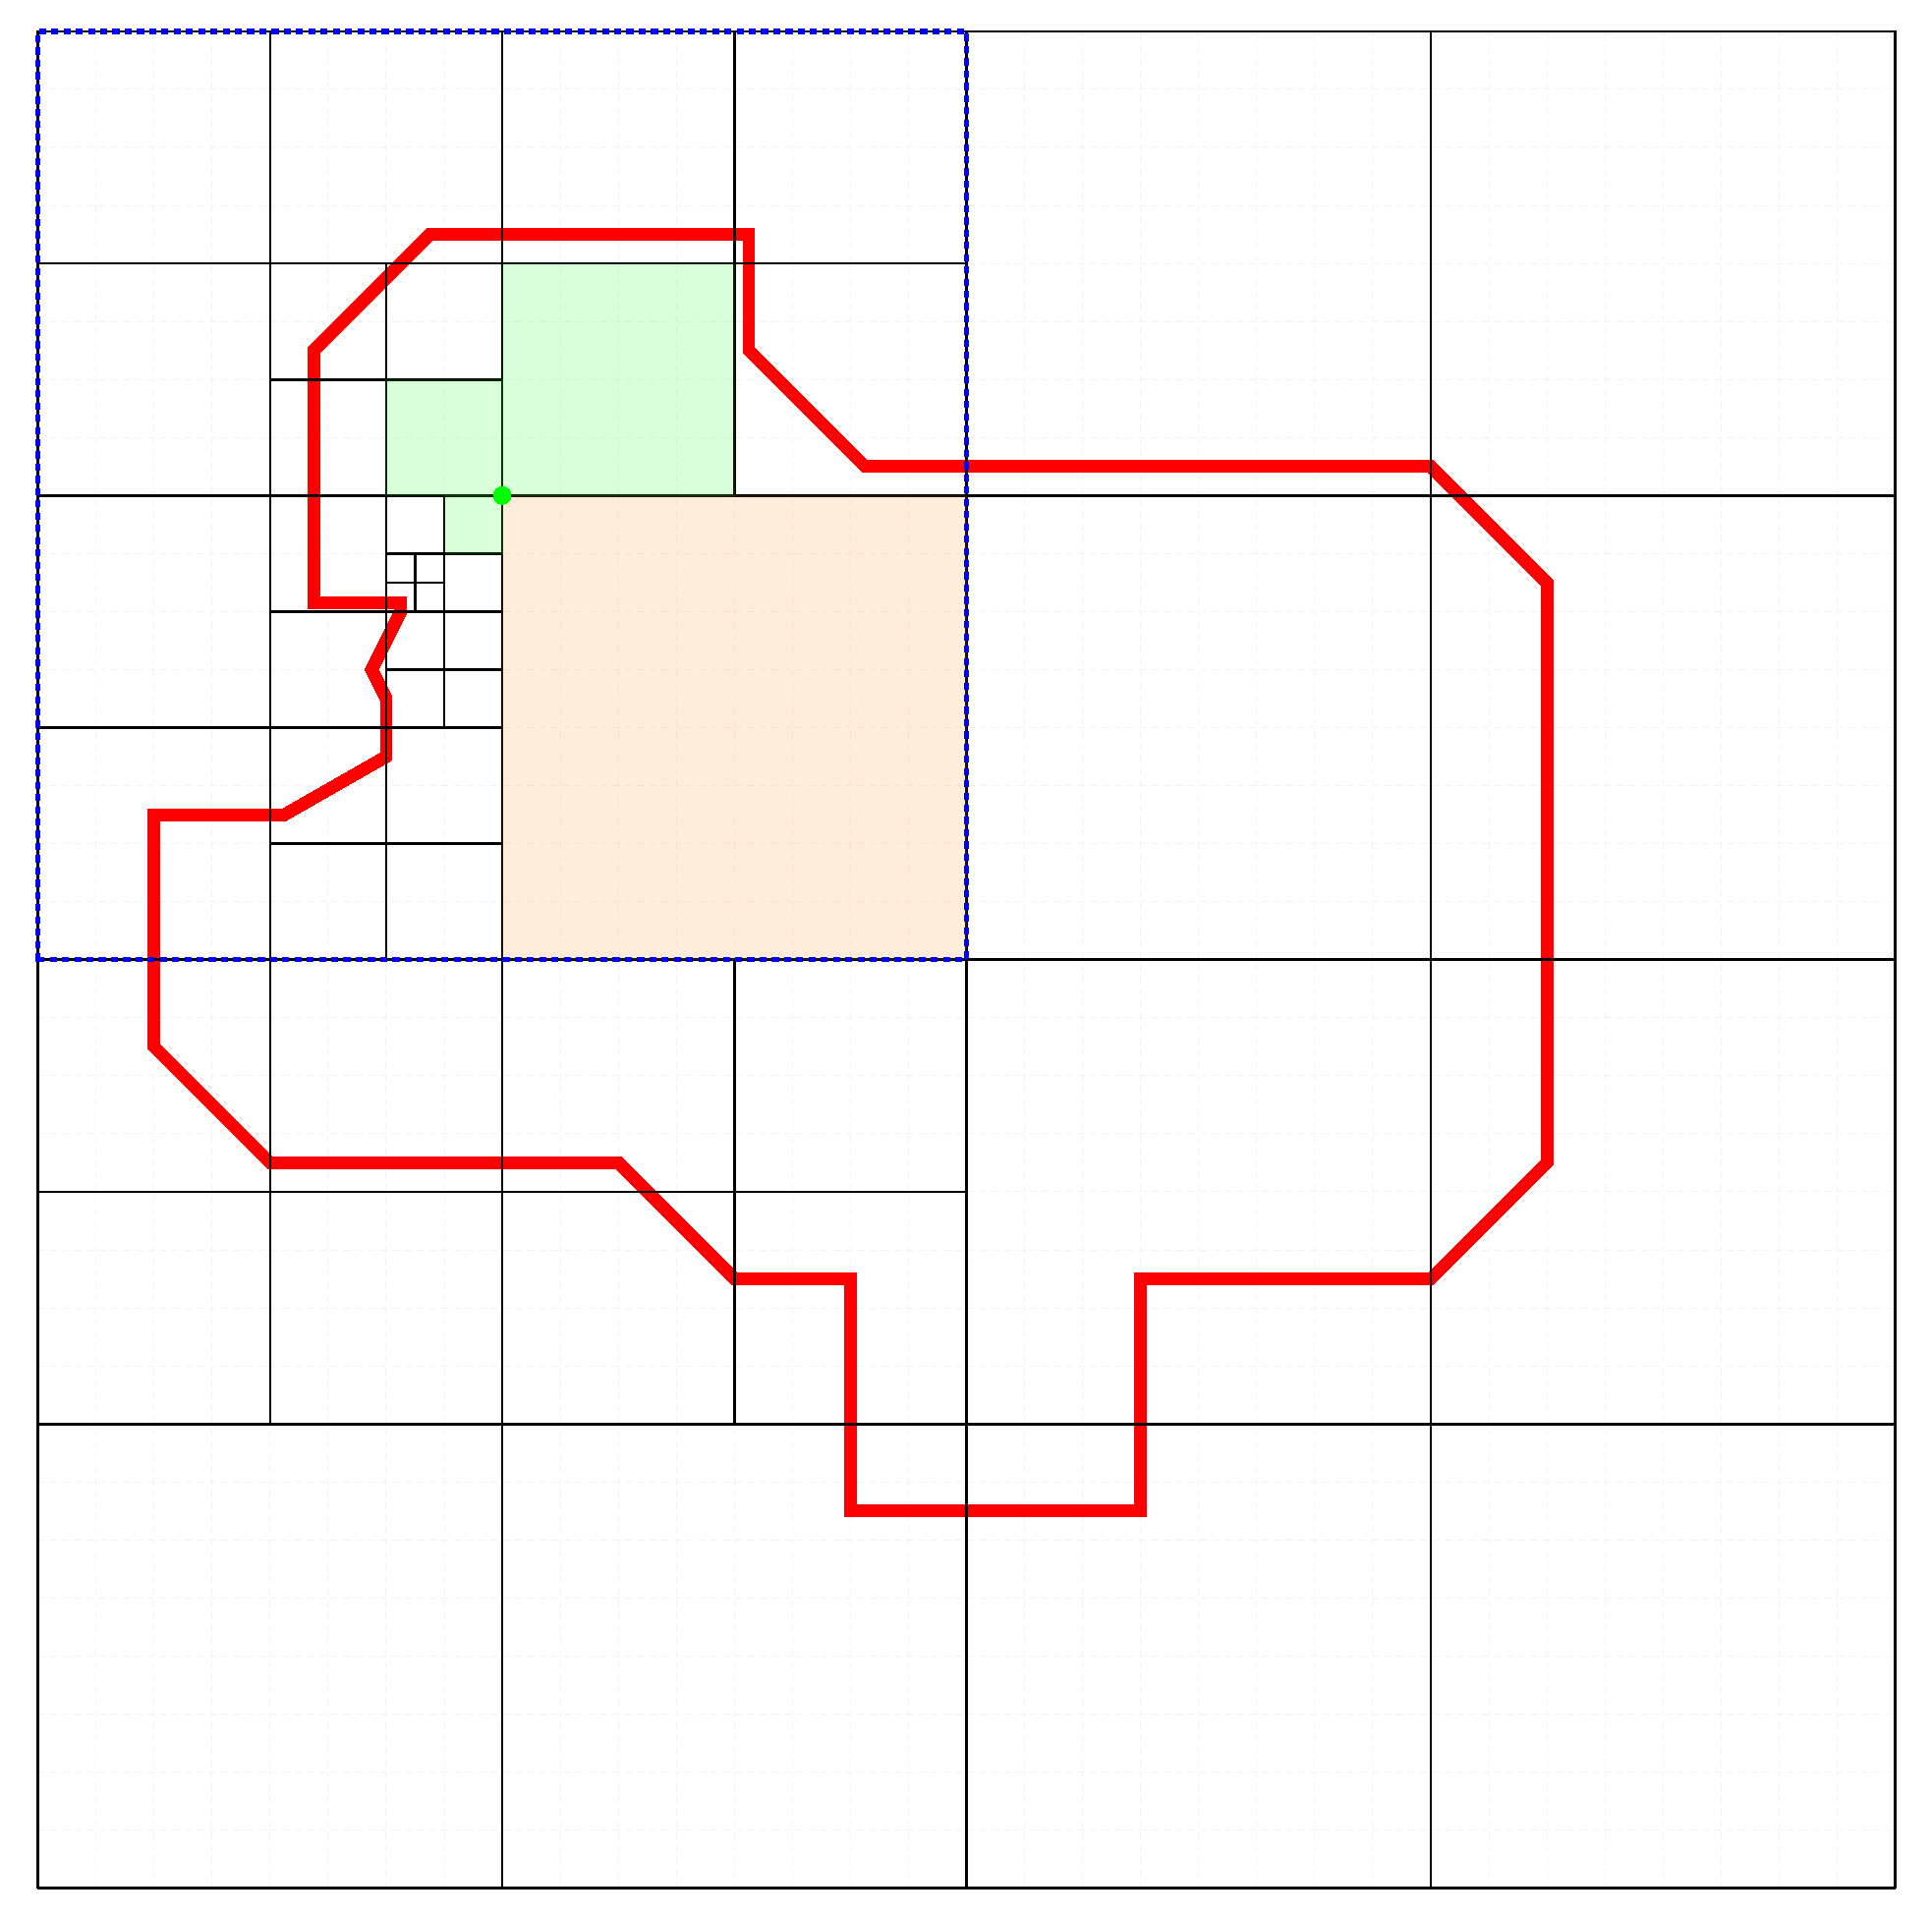
\includegraphics[page=1, width=0.24\linewidth]{figures/cellinpolygon/example}
    \includegraphics[page=2, width=0.24\linewidth]{figures/cellinpolygon/example}
    \includegraphics[page=3, width=0.24\linewidth]{figures/cellinpolygon/example}
    \caption{Three iterations of the proposed algorithm to find the next cell with valid edges from a empty cell.} \label{fig:emptycellexample}
    \Description[Iteration of the proposed algorithm]{This figure shows three iterations of the proposed algorithm to find the next cell with valid edges from a empty cell.}
\end{figure*}

The details and pseudo code of the algorithm can be seen at Algorithms \ref{alg:one} and \ref{alg:two}.  They explain the steps to obtain a near quadtree cell which guarantee the presence of edges and how select the set of three cells around of a given corner respectively.  The latter is used to choose a possible path if the current cell is empty and it needs to identify at which polygon it belongs.  The former (using the latter) ensures the finding of a cell with the polygons' edges needed to determine the enclosing polygon.

\begin{algorithm}\caption{\textsc{getNextCellWithEdges} algorithm}\label{alg:one}
    \begin{algorithmic}[1]
    \Require a quadtree with cell envelopes $\mathcal Q$ and map of cells and their edge count $\mathcal M$.
    \Function{ getNextCellWithEdges }{ $\mathcal Q$, $\mathcal M$ }
        \State $\mathcal C \gets $ list of empty cells in $\mathcal M$
        \ForEach{ $emptyCell$ in $\mathcal C $ }
            \State initialize $cellList$ with $emptyCell$ 
            \State $nextCellWithEdges \gets null$
            \State $referenceCorner \gets null$
            \State $done \gets false$
            \While{ not $done$ } 
                \State $c \gets $ last cell in $cellList$ 
                \State $cells, corner \gets \textsc{getCellsAtCorner}(\mathcal Q, c)$ \Comment{ return 3 cells and the reference corner }
                \ForEach{$cell$ in $cells$}
                    \State $nedges \gets$ get edge count of $cell$ in $\mathcal M$ 
                    \If{ $nedges > 0$ }
                        \State $nextCellWithEdges \gets cell$
                        \State $referenceCorner \gets corner$
                        \State $done \gets true$
                    \Else
                        \State add $cell$ to $cellList$
                    \EndIf
                \EndFor
            \EndWhile
            \ForEach{ $cell$ in $cellList$ }
                \State \textbf{output}($cell$, \\
                \hspace{2.5cm} $nextCellWithEdges$, $referenceCorner$)
                \State remove $cell$ from $\mathcal C$
            \EndFor
        \EndFor
    \EndFunction
    \end{algorithmic}
\end{algorithm}

\begin{algorithm} \caption{\textsc{getCellsAtCorner} algorithm}\label{alg:two}
    \begin{algorithmic}[1]
    \Require a quadtree with cell envelopes $\mathcal Q$ and a cell $c$.
    \Function{ getCellsInCorner }{ $\mathcal Q$, $c$ }
        \State $region \gets $ last character in $c.lineage$
        \Switch{ $region$ }
            \Case{ `0' }
                \State $corner \gets$ left bottom corner of $c.envelope$
            \EndCase
            \Case{ `1' }
                \State $corner \gets$ right bottom corner of $c.envelope$
            \EndCase
            \Case{ `2' }
                \State $corner \gets$ left upper corner of $c.envelope$
            \EndCase
            \Case{ `3' }
                \State $corner \gets$ right upper corner of $c.envelope$
            \EndCase
        \EndSwitch
        \State $cells \gets$ cells which intersect $corner$ in $\mathcal Q$
        \State $cells \gets cells - c$ \Comment{ Remove the current cell from the intersected cells }
        \State $cells \gets$ sort $cells$ on basis of their depth \Comment{ using $cell.lineage$ }
        \State \Return{ ($cells$, $corner$) }
    \EndFunction
    \end{algorithmic}
\end{algorithm}

We based of proposal in the following lemma and used it to proved our point with the subsequent proof.

\begin{lemma}
Four cells at the same level can not be empty.  At least one of them must have edges in order to force the split.
\end{lemma}

\begin{proof}
The $\textsc{getCellsInCorner}$ function will query the interior corner of a cell according to its position, that is the centroid of its cell parent.  The only cells which can intersect that point are cells at the same level of the current cell or their children.  If the 3 cells returned by $\textsc{getCellsInCorner}$ are empty, at least one of them must have a deeper level that the current cell.  Following that cell guarantees that the search space will be shrank at each iteration.  Eventually, the algorithm will reach the maximum level of the quadtree where all the involved cells will have the same level and, therefore, at least one of them must have edges.
\end{proof}

\subsection{Merging stage for computing final results} \label{sec:merge}
Once the distributed DCEL is ready for analysis, we have to take care on how it should be queried in order to take advantage of such distribution.  Section \ref{sec:strategy} shows the initial strategy to partition the study area and how each partition holds a section of the DCEL clipped to the cell boundary of that partition.  It is straightforward that we could query locally each of the sections but, once it is done, we should unify the results among contiguous partitions.

Faces in the interior of a partition (those which do not touch the boundary) are safe to be reported.  However, for those faces which share a half-edge with the boundary, there is a high chance that another section of that face is present in a contiguous cell and has to be checked.  

We execute a merging stage on the set of faces which touch the boundaries of each partition.  It performs a reduce operation pairing faces with the same label and dissolving their geometries.  For example, in figure \ref{fig:overlay_parted2}, it can be seen how faces in different partitions but with the same label are merged into final results by removing their common half-edges. 

\section{Overlay evaluation optimizations}\label{sec:alternative_methods}
\subsection{Optimizing for polygons expanding partitions.}\label{sec:optimizing}
To evaluate the best alternatives during the reduce/merge stage, three different approaches were evaluated to glue together segments of faces which could be located in different cells.  Those closed segments which form auto-contained faces inside of each partition are immediately reported and there is no need for additional processing.  However, those segments which touch the border of the cell in their partition must be post-processed to evaluate if they could be extended with segments in their proximity.

The first naive approach was to collect those segments in a master/root node which sequentially will combine them with the same labels and concatenate them accordingly in order to create the final and consolidated answer.  It is a straightforward method but could be really costly if the number of partitions and the subsequent number of segments touching the borders are relatively large.

As an alternative, it is proposed to do an intermediate step with a parameter introduced by the user were a level in the quadtree structure is given.  Following this parameter, the segments in partitions below the given level are collect them in intermediate nodes of the quadtree were can be evaluated partially.  The goal of this step is that part of the work can be distributed in a larger number of nodes as a previous step before to be sent to the master/root node for final evaluation.  It is expected that most of the work can be done in the intermediate step.  However, those partitions located above of the level still have to be evaluated in an individual node.

It is clear that it will create an optimization issue: if we choose a level low in the structure it can be evaluated in a larger number of intermediate nodes (taking advantage of parallelism) but, at the same time, a large number of partitions will be located above of that threshold and they will be evaluated by an unique node which can dominate the execution time.  On the other hand, if a level is selected high in the quadtree, just a few number of partitions will have to be evaluated in that unique node, but the number of intermediate nodes will also be reduced and the execution time for their evaluation will increase.

Last method take a different approach.  It partitions the set of segments at each partition by their label itself.  It is, it will reorganize the segments using their labels as the key.  The resulting dataset will put together those segments which share the same label in the same partition and they will be evaluated in the same node.  In this case, the cost of the re-partitioning should be evaluated but it is expected than the number and size of the resulting partitions will take much more advantage of parallelism.

\subsection{Optimization in the presence of unbalanced layers.}\label{sec:unbalance}
Clearly the most time consuming operation is the overlay of the individual DCELs once they have been created for each layer.  Particularly, when the combination of half-edges from each layer is performing at each cell, the most critical task is finding the intersection points between the two sets of half-edges. In many cases the number of half-edges from each layer can be quiet unbalance, it is one of the cells has much more half-edges than the other.

In the traditional approach, a common sweep-line approach is performed scanning both sets of half-edges from left to right (scanning the x-axis) inside each cell and the corresponding intersections points are reported in order to continue with the creation of the merged DCEL (see Section \ref{sec:prelim}). This approach does not consider the fact that in some cells, one of the sets can be larger than the other and there is no need to scan all the half-edges in many cases.

An alternative approach is proposed for those cases.  It start detecting which set contains more half-edges and which has more probability to overlap the smaller one in the x-axis. Then, it performs a simple scan in the smaller to extract the wide of this dataset and returned in the form of intervals over the x-axis.  It has to be noted that a smaller dataset can extend in several intervals over the bigger dataset and it has been managed accordingly.  

With each interval, it is possible to locate the point in the x-axis where the sweep-line algorithm should start scanning from the bigger set and compared with the half-edges from de smaller one. On those cases where the bigger and smaller set differ considerably in size, it is possible to save time due to the fact that many sections of the bigger set do not required to be scanned nor compared with the smaller set.
\section{Experimental Evaluation} \label{sec:experiments}

For our experimental evaluation, we used a 12-node Linux cluster (kernel 3.10) and Apache Spark 2.4. Each node has 9 cores (each core is an Intel Xeon CPU at 1.70GHz) and 2G memory.

\textbf{Evaluation datasets}.
The details of the real datasets of polygons that we use are summarized in Table \ref{tab:datasets}. The first dataset (MainUS) contains the complete Census Tracts for all the states on the US mainland for the years 2000 (layer A) and 2010 (layer B). It was collected from the official website of the United States Census Bureau\footnote{\url{https://www2.census.gov/geo/tiger/TIGER2010/TRACT/}}. The data was clipped to select just the states inside the continent. Something to note with this dataset is that the two layers present a spatial gap (which was due to improvements in the precision introduced for 2010). As a result, there are considerably more intersections between the two layers, thus creating many new faces for the DCEL.

The second dataset, GADM - taken from Global Administration Areas\footnote{\url{https://gadm.org/}}, collects the geographical boundaries of the countries and their administrative divisions around the globe. For our experiments, one layer selects the States (administrative level 2), and the other has Counties (administrative level 3). Since GADM may contain multi-polygons, we split them into their individual polygons. 

Since these two datasets are too large, a third, smaller dataset was created for comparisons with the sequential algorithm. This dataset is the California Census Tracts (CCT), a subset from MainUS for the state of California; layer A corresponds to the CA census tracts from the year 2000, while layer B corresponds to 2010. Below, we also use other states to create datasets with different numbers of faces.  
To test the scalable approach, a sequential algorithm for DCEL creation was implemented based on the pseudo-code outlined in \cite{berg_computational_2008}.

\begin{table}
    \small
    \caption{Evaluation Datasets}
    \label{tab:datasets}
    \begin{tabular}{c c c c}
        \toprule
        Dataset & Layer & Number        & Number    \\
                &       & of polygons   & of edges  \\
        \midrule
        MainUS& Polygons for 2000 & 64983 & 35417146        \\
              & Polygons for 2010 & 72521 & 36764043        \\
        GADM  & Polygons for Level 2 & 160241 & 64598411    \\
              & Polygons for Level 3 & 223490 & 68779746    \\
        CCT   & Polygons for 2000 & 7028 & 2711639          \\
              & Polygons for 2010 & 8047 & 2917450          \\
        \bottomrule
    \end{tabular}
\end{table}

The scalable approach was implemented over the Apache Spark framework.  From a Map-Reduce point of view the stages described in Section  \ref{sec:methods} were implemented using several transformations and actions supported by Spark.  For example, the partitioning and load balancing described in Section \ref{sec:pstrategies} and \ref{sec:partitioning_ddcel} was implemented using a Quadtree, where its leaves were used to map and balance the number of edges that have to be sent to the worker nodes.  Mostly, map operations were used to process and locate the edges in the corresponding leaf to exploit proximity among them while at the same time dividing the amount of work among worker nodes.
Similarly, the edges at each partition were processed using chains of transformations at local level (see Section \ref{sec:methods}) followed by reducer actions to post-process incomplete faces which could span over multiples partitions and have to be combined or re-distributed to obtain the final answer.  In addition, the reduce actions were further optimized as described in Section \ref{sec:alternative_methods}.

\subsection{Overlay face optimizations}\label{sec:overlay_optimization}
We first examine the optimizations in Section \ref{sec:optimizing}. To consider different distributions of faces, for these experiments, we used 8 states from the MainUS dataset with different numbers of tracts (faces). In particular, we used, in decreasing order of number of tracts, CA, TX, NC, TN, GA, VA, PA, and FL. For each state, we computed the distributed overlay between two layers (2000 and 2010). For each computation, we compared the baseline; master at the root node, with intermediate reducers at different levels: $i$ varied from 4 to 10. 

Figure \ref{fig:overlay_tester} shows the results for the distributed overlay computation stage; after the local DCELs were computed at each cell. 
Note that for each state experiment, we tested different numbers of cells for the quadtree and reported the configuration with the best performance. To determine this, we sampled 1\% of the edges for each state and evaluated the best number of cells ranging from 200 to 2000. In most cases, the best number of cells was around 3000.
As expected, there is a trade-off between parallelism and how much work is left to the final reduce job. For different states, the optimal $i$ varied between levels 4 and 6. The figure also shows the optimization that re-partitions the faces by label id. This approach has actually the best performance. This is because few faces with the same label can be combined independently. This results in smaller jobs better distributed among the cluster nodes, and no reduce phase is needed. As a result, we use the label re-partition approach for the rest of the experiments to implement the overlay computation stage.

Finally we note that the overlay face optimizations involve shuffling of the incomplete faces. Table \ref{tab:percentages} shows the percentage of incomplete faces for three states, assuming 3000 cells. As it can be seen, the incomplete faces is small (in average 12.89\%) and moreover, for the \textit{By Label} approach, this shuffling is parallelized.

\begin{table}
    \centering
    \caption{Percentages of edges in incomplete faces for three states} \label{tab:percentages}
    \begin{tabular}{cccc}
        \hline
                & Number of & Edges in         &            \\
        Dataset & edges     & incomplete faces & Percentage \\
        \hline
        CA &  47834 &  6339 & 13.25\% \\
        TX &  41227 &  4436 & 10.75\%\\
        FL &  24152 &  3547 & 14.68\%\\
        \hline
    \end{tabular}
\end{table}

\begin{figure}
    \centering
    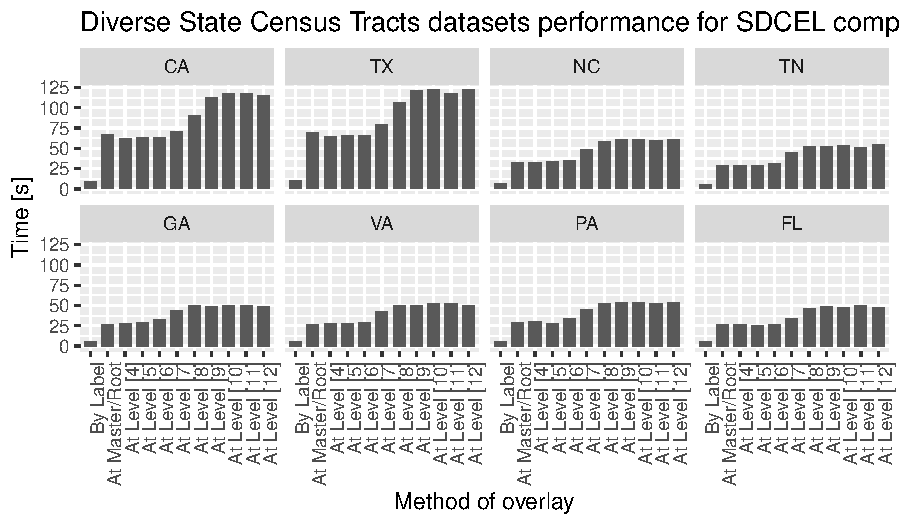
\includegraphics[width=\linewidth]{Overlay_Tester}
    \caption{Overlay methods evaluation.}\label{fig:overlay_tester}
\end{figure}

\subsection{Unbalanced layers optimization}

For these experiments, we compared the traditional sweep approach with the `filtered-sweep' approach that considers only the areas where the smaller layer has edges (Section \ref{sec:unbalance}).  To create the smaller cell layer, we picked a reference point in the state of Pennsylvania, from the MainUS dataset, and added 2000 census tracts until the number of edges reached 3K. We then varied the size of the larger cell layer in a controlled way: using the same reference point but using data from the 2010 census, and we started adding tracts to create a layer that had around 2x, 3x, ..., 7x the number of edges of the smaller dataset. 

Since this optimization occurs per cell, we used a single node to perform the overlay computation within that cell. Figure \ref{fig:unbalance_tests}(a) shows the behavior of the two methods (filtered-sweep vs. traditional sweep) under the above-described data for the overlay computation stage.  Clearly, as the data from one layer grows much larger than the other layer, the filtered-sweep approach overcomes the traditional one.

\begin{figure}
    \centering
    \begin{tabular}{cc}
       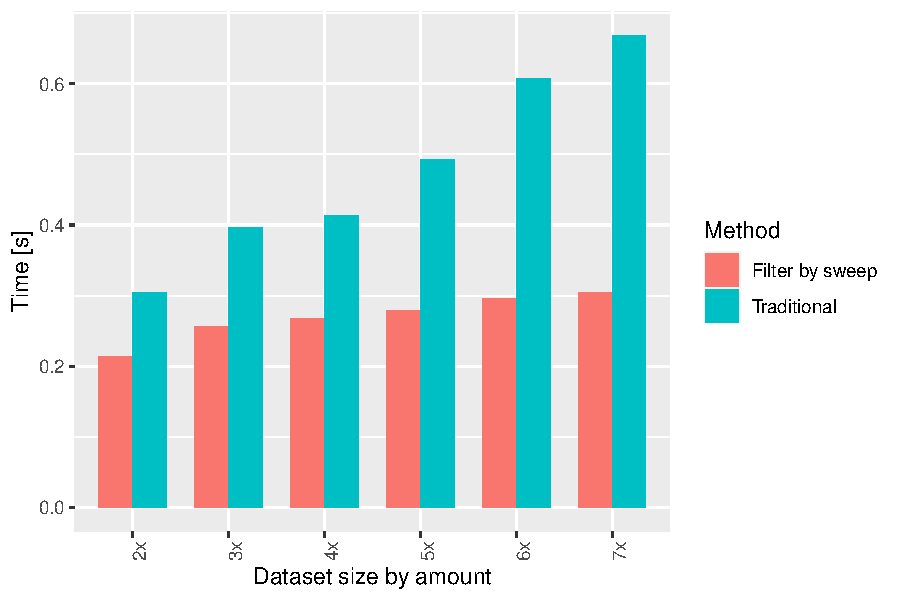
\includegraphics[width=0.49\linewidth]{Unbalance_Tester01}  & 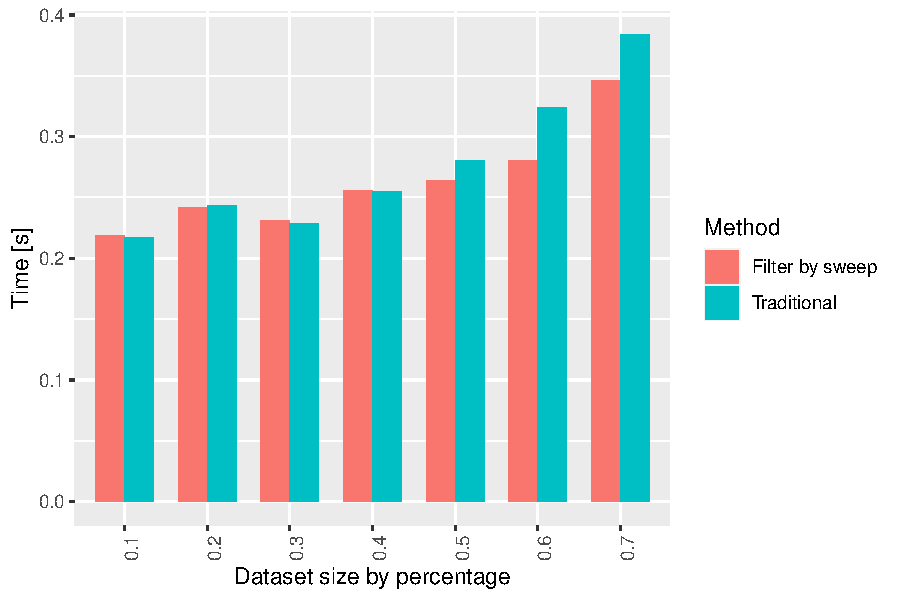
\includegraphics[width=0.49\linewidth]{Unbalance_Tester02} \\
       (a) & (b)
    \end{tabular}
    \caption{Evaluation of the unbalanced layers optimization.}\label{fig:unbalance_tests}
\end{figure}

We also performed an experiment where the difference in size between the two layers varies between 10\% and 70\%. For this experiment, we first identified cells from the GADM dataset where the smaller layer had around 3K edges. Among these cells, we then identified those where the larger layer had 10\%, 20\%, ... up to 70\% more edges. In each category, we picked 10 representative cells and computed the overlay for the cells in that category.  

Figure \ref{fig:unbalance_tests}(b) shows the results; in each category, we show the average time to compute the overlay among the 10 cells in that category. The filtered-sweep approach shows better performance as the percentage difference between layers increases. Based on these results, one could apply the optimization on those cells where the layer difference is significant (more than 50\%).
We anticipate that this optimization will be particularly beneficial for datasets where the two input layers contain many cells with significantly different edge counts.

\subsection{Varying the number of cells}
The quadtree configuration allows for performance tuning by setting the \textit{maximum capacity} of a cell. The quadtree continues splitting until this capacity is reached. There is an inverse relationship between the capacity and the number of leaf cells: a lower capacity results in more cells, while a higher capacity leads to fewer leaf cells. In skewed datasets, the quadtree may become unbalanced, with some branches splitting more frequently. As a result, the final number of partitions is not necessarily a multiple of four. In the figures, we round the number of leaf cells to the nearest thousand.

The number of cells affects the performance of our scalable overlay implementation, termed as SDCEL, since it relates to the average cell capacity given by the number of edges it could contain. As it was said before, a fewer number of cells implies larger cell capacity and thus more edges to process within each cell. Complementary, creating more cells increases the number of jobs to be executed.  

Figure \ref{fig:ca}(a) shows the SDCEL performance using the two layers of the CCT dataset while varying the number of cells from 100 to 15K (by multiple of 1000). Each bar corresponds to the time taken to create the DCEL for each layer and then combine them to create the distributed overlay. Clearly, there is a trade-off: as the number of cells increases, the SDCEL performance improves until a point where the larger number of cells adds an overhead. Figure \ref{fig:ca}(b) focuses on that area; the best SDCEL performance was around 7K cells.

In addition, Figure \ref{fig:ca}(a) shows the performance of the sequential solution (CGAL library) for computing the overlay of the two layers in the CCT dataset using one of the cluster nodes. Clearly, the scalable approach is much more efficient as it takes advantage of parallelism. Note that the CGAL library would crash when processing the larger datasets (MainUS and GADM).

\begin{figure}
    \centering
    \begin{tabular}{cc}
        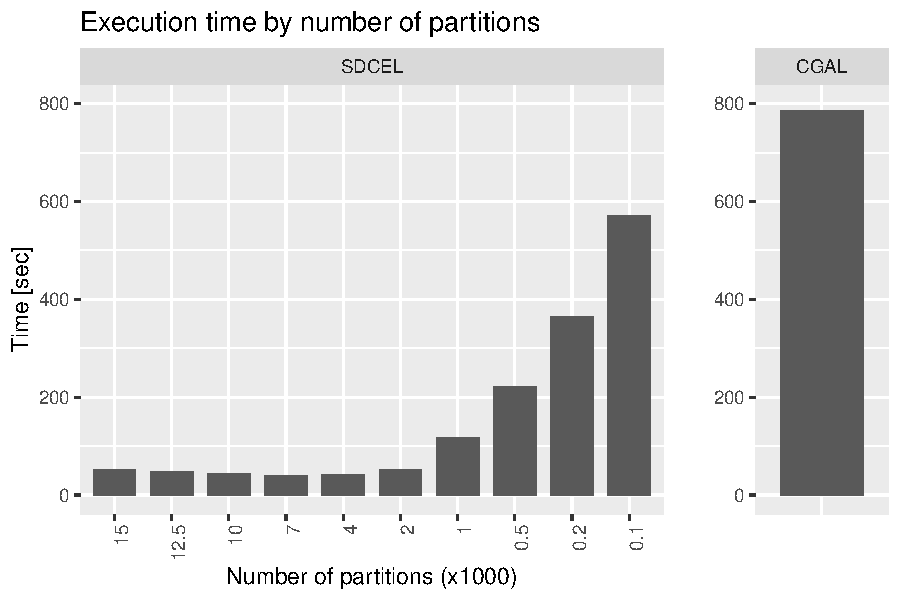
\includegraphics[width=0.50\linewidth]{CA} & 
        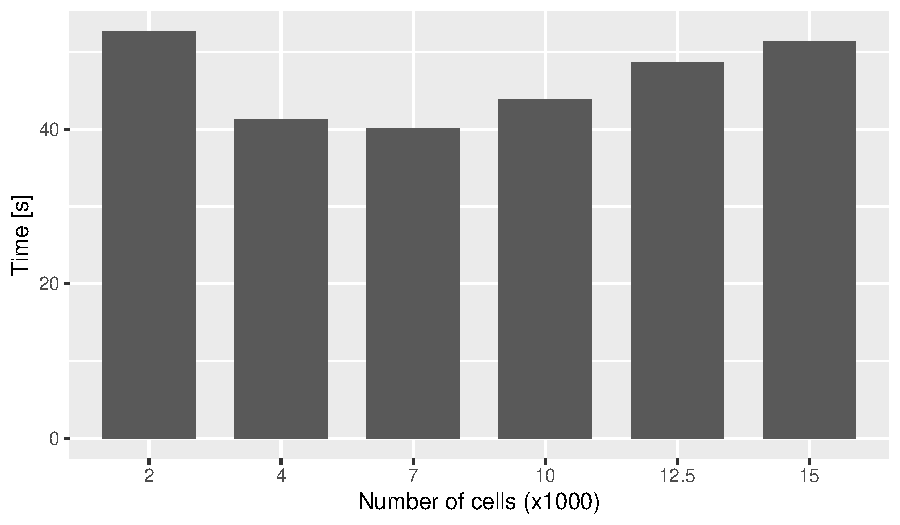
\includegraphics[width=0.45\linewidth]{CA_sample} \\
        (a) & (b)
    \end{tabular}
    \caption{SDCEL performance while varying the number of cells in the CCT dataset.} \label{fig:ca}
\end{figure}

\begin{figure}
    \centering
    \begin{tabular}{cc}
        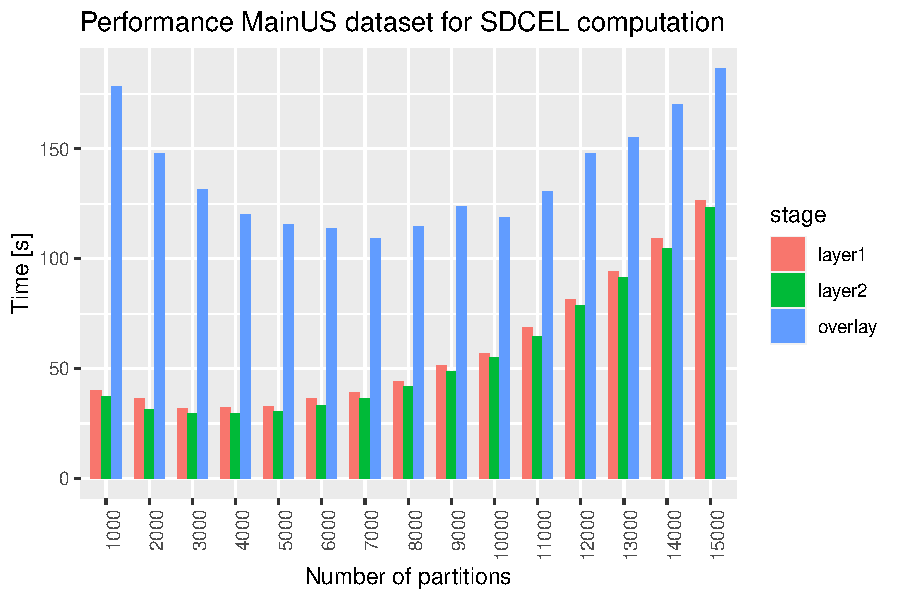
\includegraphics[width=0.49\linewidth]{MainUS} &
        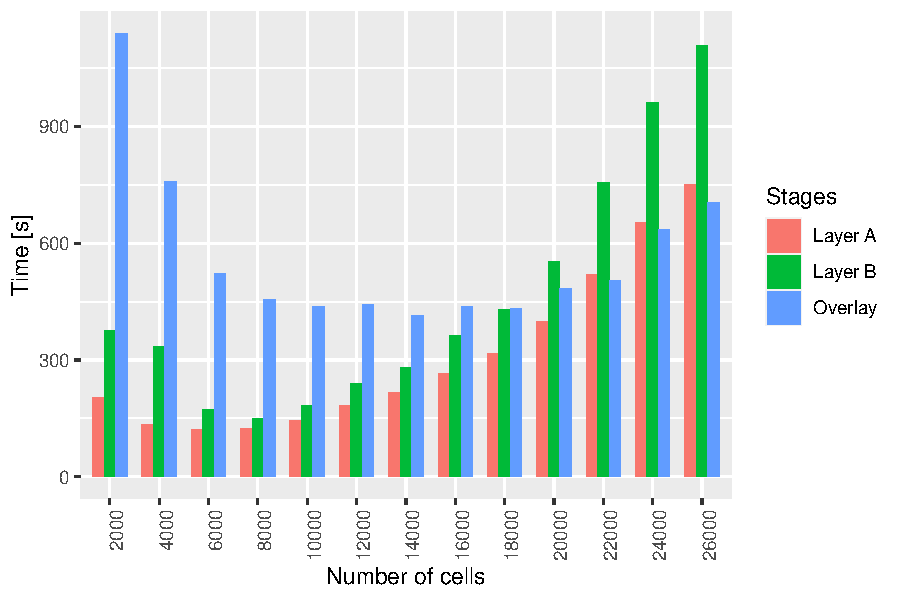
\includegraphics[width=0.49\linewidth]{GADM}   \\
        (a) & (b)
    \end{tabular}
    \caption{Performance with (a) MainUS and (b) GADM datasets.} \label{fig:mainus}
\end{figure}

Figure \ref{fig:mainus} shows the results when using the larger MainUS and GADM datasets, while again varying the number of cells parameter from 8K to 18K and from 16K to 34K, respectively. In this figure, we also show the time taken by each stage of the overlay computation.  This is, the time to create the DCEL for layer A, for layer B, and for their combination to create their distributed overlay. We can see a similar trade-off in each of the stages. The best performance is given when setting the number of cells parameter to 12K for the MainUS and 22K for the GADM dataset. Note that in the MainUS dataset, the two layers have a similar number of edges; as can be seen, their DCEL computations are similar.  

Interestingly, the overlay computation is expensive since as mentioned earlier there are many intersections between the two layers. An interesting observation from the GADM plots is that layer B takes more time than layer A; this is because there are more edges in the counties than in the states. Moreover, county polygons are included in the (larger) state polygons. When the size of cells is small (i.e., a larger number of cells like in the case of 34K cells), these cells mainly contain counties from layer B. As a result, there are not many intersections between the layers in each cell, and the overlay computation is thus faster. On the other hand, with large cell sizes (smaller number of cells), the area covered by the cell is larger, containing more edges from states and thus increasing the number of intersections, resulting in higher overlay computation.

Additionally, Table \ref{tab:cell_stats} provides statistics on the cells. It shows that in larger datasets, an average cell size of approximately 3000 edges produces the best results. This cell size ensures a relatively small amount of data to transmit, which minimizes the impact on data shuffling and processing.
Table \ref{tab:orphans} presents the number of cells, original holes, and the orphan cells and holes generated after partitioning.

\begin{table}
    \centering
    \caption{Cell size statistics.}
    \label{tab:cell_stats}
    \begin{tabular}{ccccccc}
        \hline
        Dataset & Min & 1st Qu. & Median & Mean & 3rd Qu. & Max   \\
        \hline
        GADM    & 0   & 0       & 2768   & 3141 & 5052    & 16978 \\
        MainUS  & 0   & 1538    & 2582   & 2853 & 3970    & 10944 \\
        CCT     & 0   & 122     & 324    & 390  & 546     & 1230  \\
        \hline
    \end{tabular}
\end{table}

\begin{table}
    \small
    \caption{Orphan cells and orphan holes description}
    \label{tab:orphans}
    \begin{tabular}{c c c c}
        \toprule
                &          &          & Number       \\
                & Number   & Number   & of orphans   \\
        Dataset & of cells & of holes & (cell/holes) \\
        \midrule
        GADM  & 21970      & 1999     & 4310 \\
        MainUS& 12343      & 850      & 1069 \\
        CCT   & 7124       & 40       & 215  \\
        \bottomrule
    \end{tabular}
\end{table}

\subsection{Speed-up and Scale-up experiments}\label{sec:speed_scale}

The speed-up behavior of SDCEL appears in Figure \ref{fig:mainus_speed_scale}(a) (for the MainUS dataset) and in Figure \ref{fig:gadm_speed_scale}(a) (for the GADM dataset); in both cases, we show the performance for each stage. For these experiments, we varied the number of nodes to 3, 6, and 12 while keeping the input layers the same. Clearly, as the number of nodes increases, the performance improves. SDCEL shows good speed-up characteristics: as the number of nodes doubles from 3 to 6 and then from 6 to 12, the performance improves by almost half. 

\begin{figure}
    \centering
    \begin{tabular}{cc}
       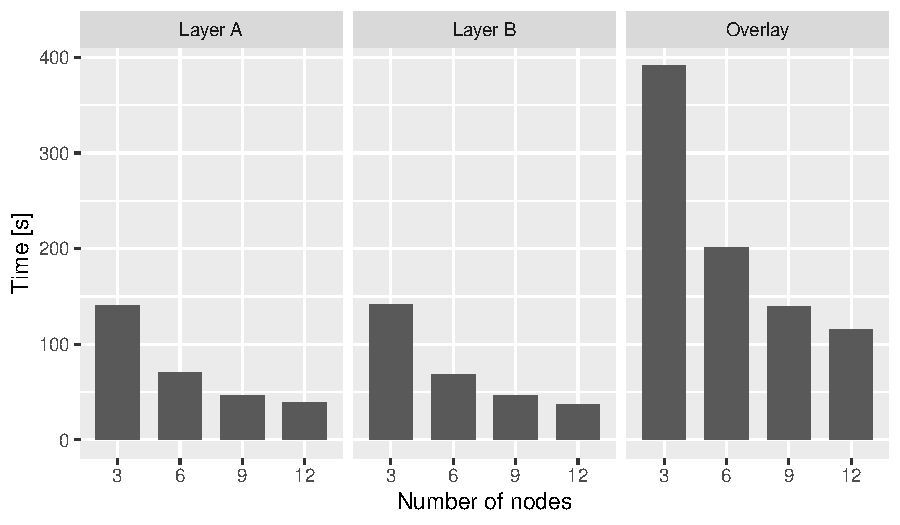
\includegraphics[width=0.49\linewidth]{MainUS_speedup} & 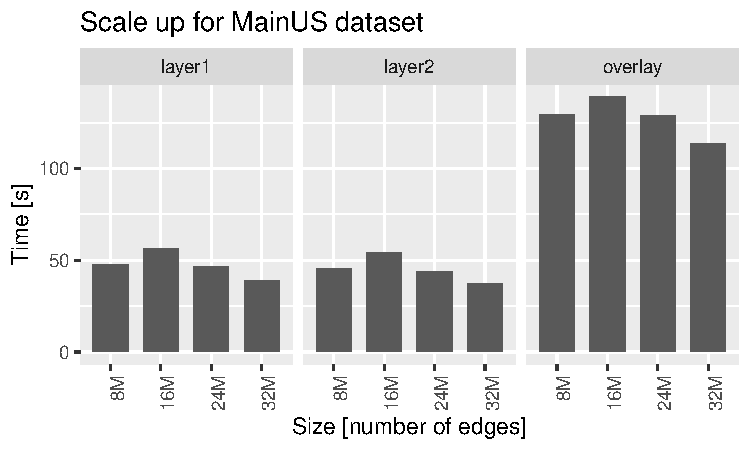
\includegraphics[width=0.49\linewidth]{MainUS_scaleup} \\
       (a) & (b)
    \end{tabular}
    \caption{Speed-up and Scale-up experiments for the MainUS dataset.} \label{fig:mainus_speed_scale}
\end{figure}

\begin{figure}
    \centering
    \begin{tabular}{cc}
       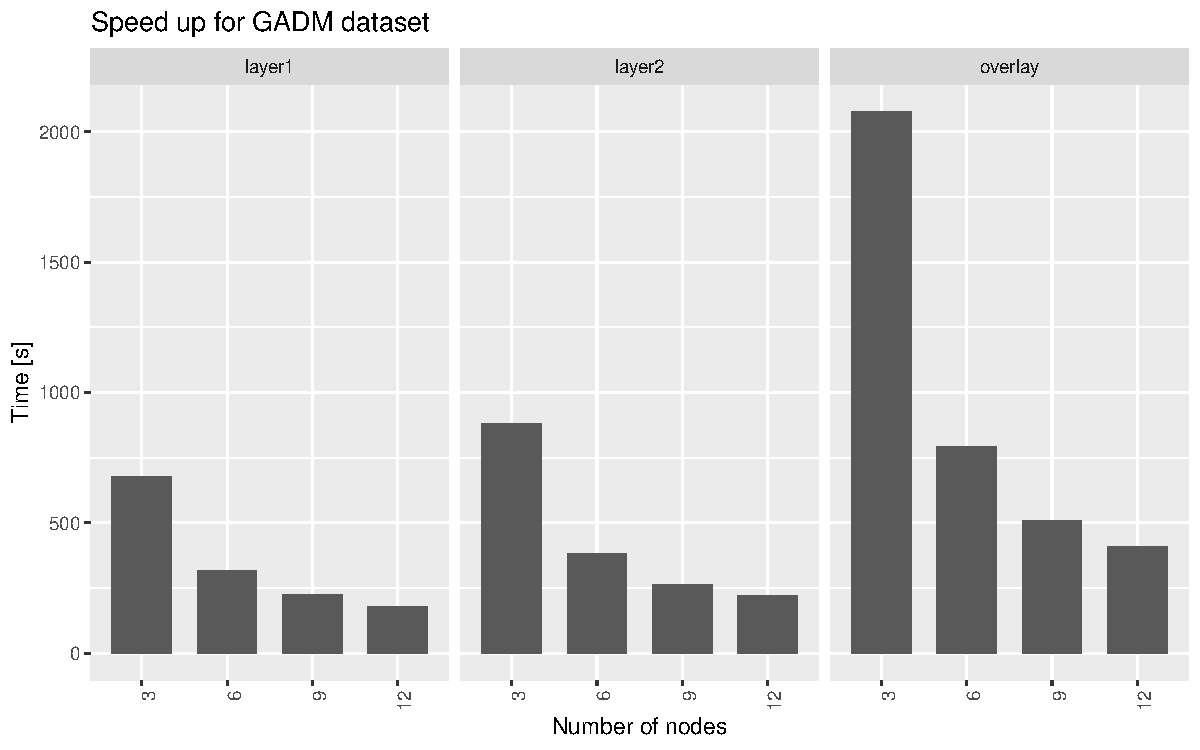
\includegraphics[width=0.49\linewidth]{GADM_speedup} & 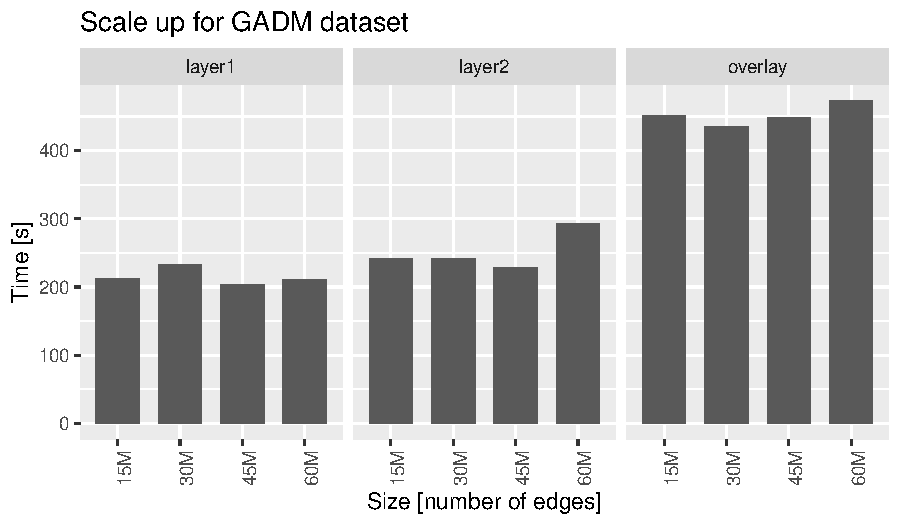
\includegraphics[width=0.49\linewidth]{GADM_scaleup} \\
       (a) & (b)
    \end{tabular}
    \caption{Speed-up and Scale-up experiments for the GADM dataset.} \label{fig:gadm_speed_scale}
\end{figure}

To examine the scale-up behavior, we created smaller datasets out of the MainUS and similarly out of the GADM so that we could control the number of edges. To create such a dataset, we picked a centroid and started increasing the area covered by this dataset until the number of edges was closed to a specific number. For example, from the MainUS, we created datasets of sizes 8M, 16M, and 32M edges for each layer. We then used two layers of the same size as input to a different number of nodes while keeping the input-to-node ratio fixed. That is, the layers of size 8M were processed using 3 nodes, the layers of size 16M using 6 nodes, and the 32M using 12 nodes. We used the same process for the scale-up experiments with the GADM dataset. The results appear in Figure \ref{fig:mainus_speed_scale}(b) and Figure \ref{fig:gadm_speed_scale}(b).  Overall, SDCEL shows good scale-up performance; it remains almost constant as the work per node is similar (there are slight variations because we could not control perfectly the number of edges and their intersection). 


\subsection{Kd-tree versus quadtree performance}
\label{sec:comparison}

In order to compare the quadtree and the kd-tree partition strategies we analyze their performance during the construction of the spatial data structure which defines the cells that the partition will use based on the sample, the cost of partitioning; populating the cells with the full datasets, and the overall time to complete the phases of the overlay operation using each partitioning approach. 
%In this section, we compare the performance of the quadtree and kd-tree partition strategies in the phases mentioned above and the number of nodes used by each structure.  
We use the datasets of MainUS and GADM described in Table \ref{tab:datasets}.

\begin{figure}
    \centering
    \begin{tabular}{cc}
        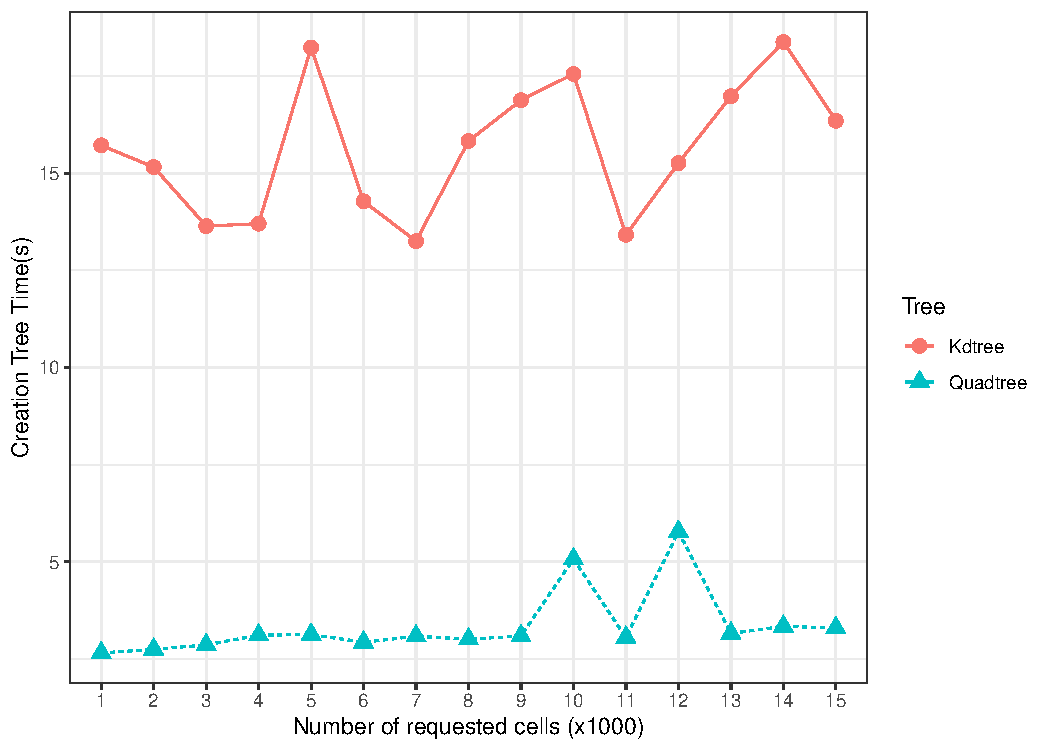
\includegraphics[width=0.49\linewidth]{K_Creation_US.pdf} & 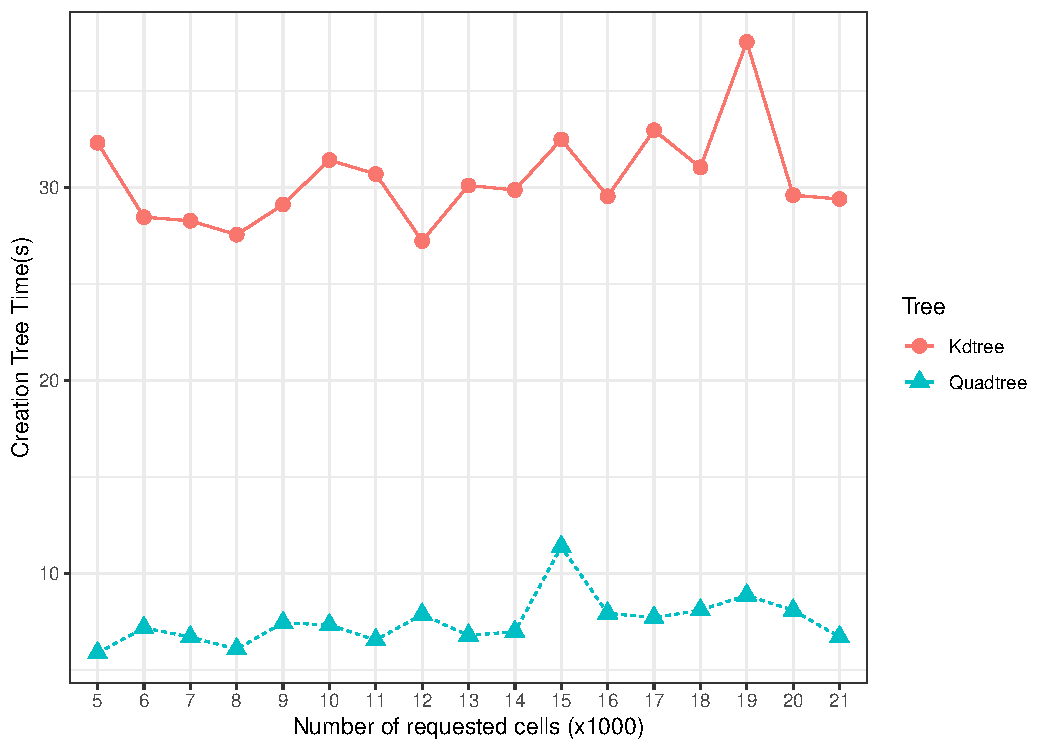
\includegraphics[width=0.49\linewidth]{K_Creation_GADM.pdf} \\
        (a) & (b) 
    \end{tabular}
    \caption{Construction time for the spatial data structure in the (a) MainUS and (b) GADM datasets.} \label{fig:k_creation_us}
\end{figure}


\begin{figure}
    \centering
    \begin{tabular}{cc}
        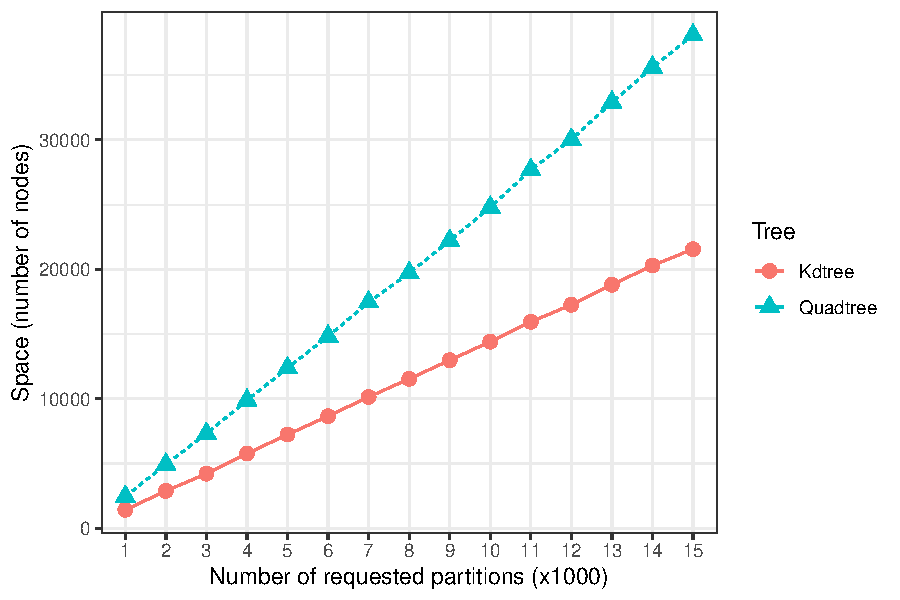
\includegraphics[width=0.49\linewidth]{K_Space_US.pdf} & 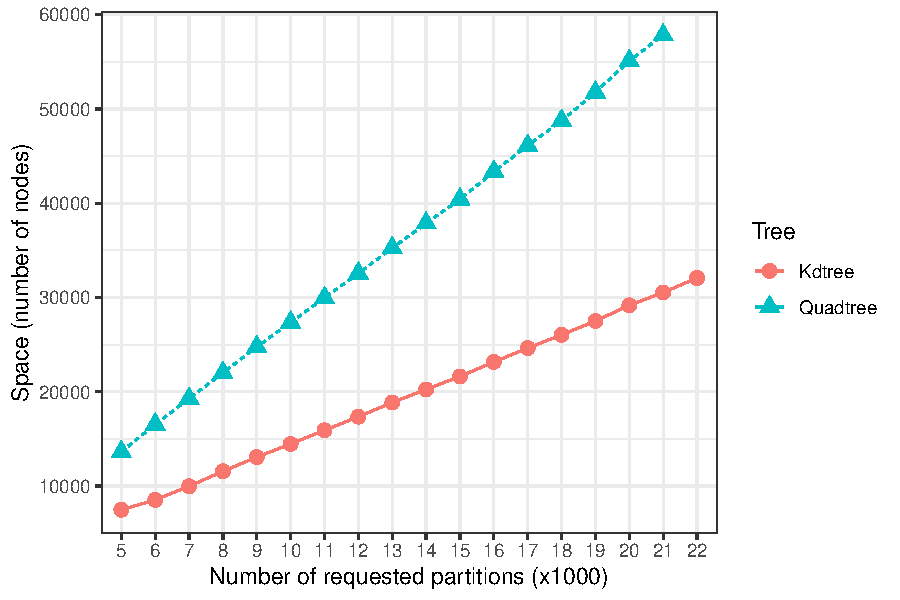
\includegraphics[width=0.49\linewidth]{K_Space_GADM.pdf} \\
        (a) & (b) 
    \end{tabular}
    \caption{Number of cells created by each spatial data structure in the (a) MainUS and (b) GADM datasets.} \label{fig:k_space_us}
\end{figure}

Figure \ref{fig:k_creation_us} depicts the construction time during the sampling of the input layers and the generation of the partitioning cells after requesting a different number of divisions. We can see that the kd-tree takes more time, particularly because of the sorting done at each split, so as to organize the data and localize the middle point. 
In average, Quadtree takes 23.13\% the time it takes for Kdtree to be created (21.55\% in MainUS and 24.72\% in GADM). However, the Kdtree creation is just 5.86\% of the overall time during the total DCEL construction (6.88\% in MainUS and 4.87\% in GADM).

\begin{figure}
    \centering
    \begin{tabular}{cc}
        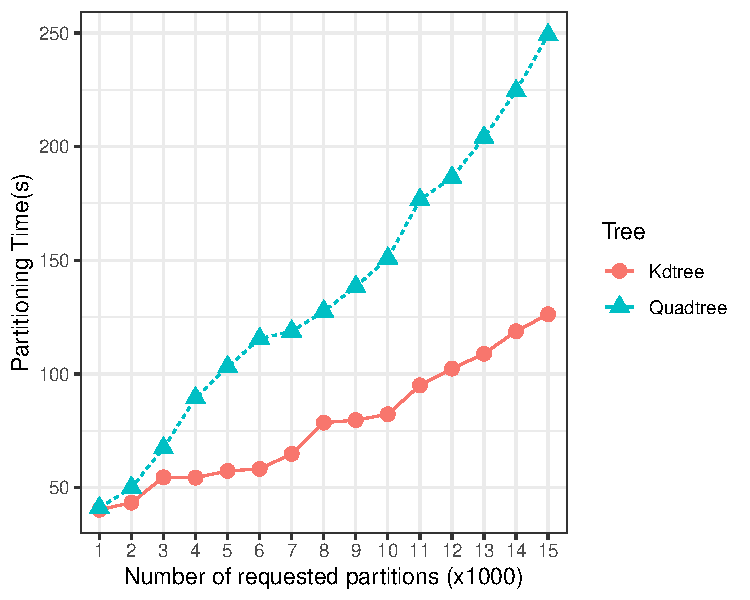
\includegraphics[width=0.49\linewidth]{K_Partitioning_US.pdf} & 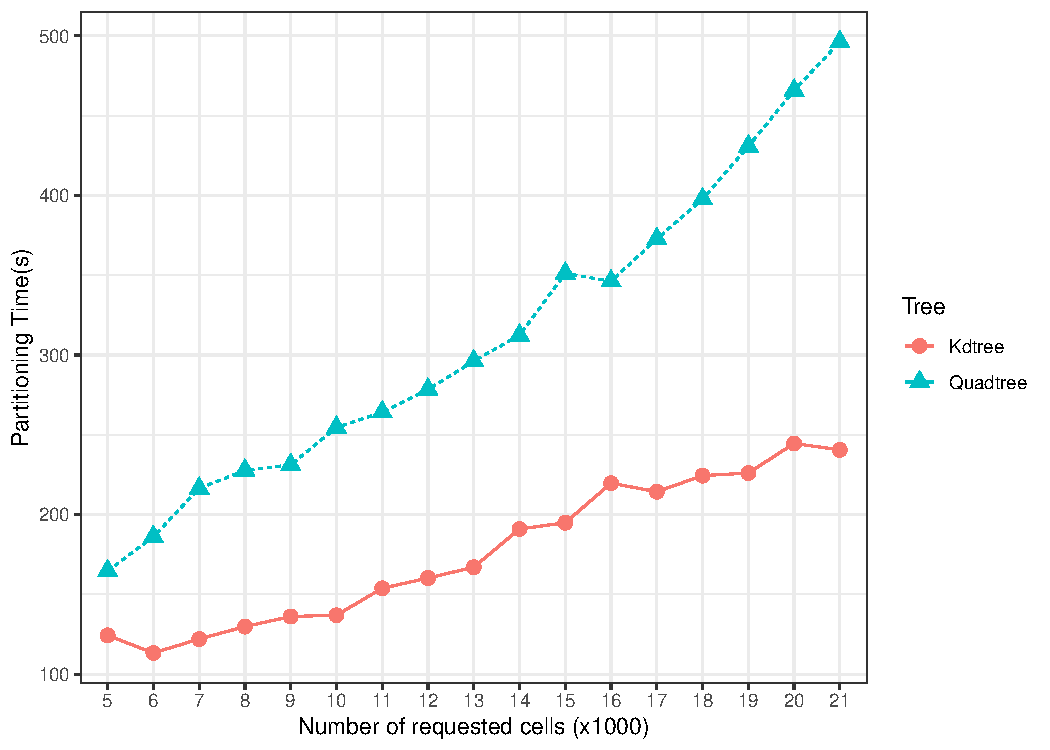
\includegraphics[width=0.49\linewidth]{K_Partitioning_GADM.pdf} \\
        (a) & (b) 
    \end{tabular}
    \caption{Data partitioning time using a spatial data structure (a) in the MainUS dataset and (b) in the GADM dataset.} \label{fig:k_partitioning_us}
\end{figure}

An important characteristic of the behavior of each partitioning scheme is the number of cells (partitions) each sample data structure creates. 
Figure \ref{fig:k_space_us} depicts the number of cells created by each spatial data structure. As the quadtree follows a space-oriented technique, it creates more nodes (4 at each split) and thus generates more leaves (cells); more of them are prone to be empty compared to the kd-tree. 

Figure \ref{fig:k_partitioning_us} shows the cost to partition the full content of both layers. Given a sample tree data structure, each edge is assigned to a cell (partition) depending on which leaf the edge is located; edges are assigned (copied) to all leaves they intersect. Then, a shuffle operation is performed to move the data to the corresponding node that will handle this cell (partition). This figure shows that the quadtree partitioning takes more time. This depends largely on the number of leaves created by the sample tree and the number of edges that overlap partitions (which is expected to be larger for the quadtree since it uses more and thus smaller cells). 

%As we will see the Quadtree partitioning creates many more leaves, affecting the number of cells used.

\begin{figure}
    \centering
    \begin{tabular}{cc}
        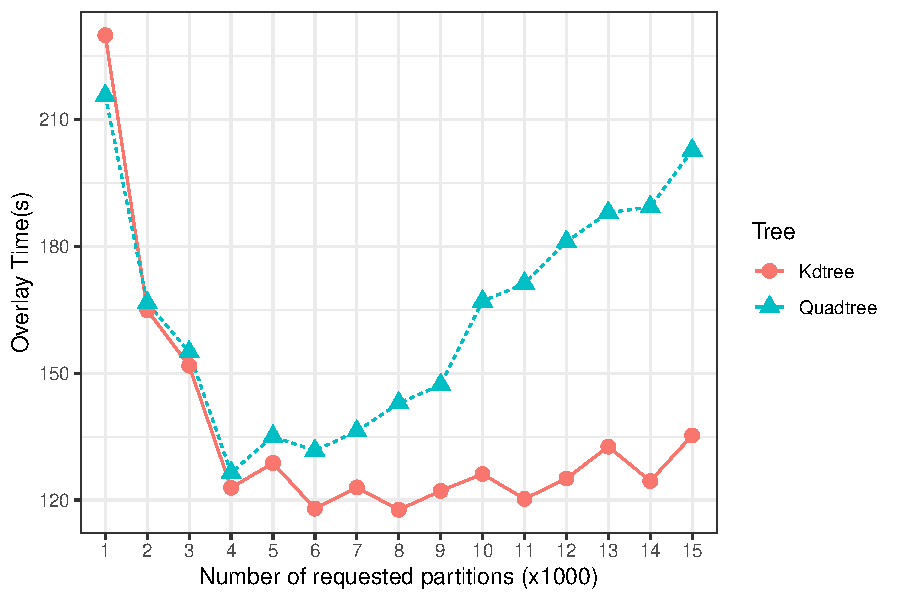
\includegraphics[width=0.49\linewidth]{K_Overlay_US.pdf} & 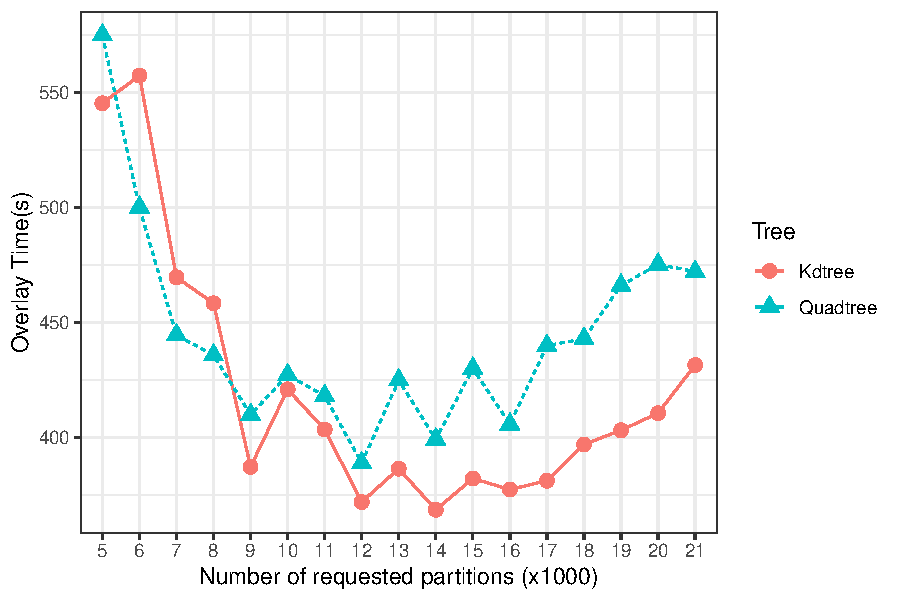
\includegraphics[width=0.49\linewidth]{K_Overlay_GADM.pdf} \\
        (a) & (b) 
    \end{tabular}
    \caption{Execution time for the overlay operation using a spatial data structure in the MainUS (a)and GADM (b) dataset.} \label{fig:k_overlay_us}
\end{figure}

Once the data is assigned to their partitions, the overlay operation can be executed.  Figure \ref{fig:k_overlay_us} shows the overlay performance under each partition strategy, for different number of cells. The Kd-tree approach performs better; as the quadtree tends to generate more and emptier cells, its performance is directly affected.

As it was said before, in particular on partitioning based on Kdtree, the smaller number of cells/partitions used in this approach give also an improvement on the impact of shuffling during the partition strategy because the number and size of the resulting partitions have a lower impact into the communication cost.

Finally, we consider the speed-up and scale-up performance using the kd-tree partitioning. Figure \ref{fig:k_scale_speed_us}(a) shows the speed-up performance using the MainUS dataset (36M edges) while varying the number of nodes (for 3, 6, and 12 nodes). Similar to the quadtree partitioning strategy, the kd-tree partitioning shows good speed-up performance. As resources duplicate the execution time improves almost by a half. 

Figure \ref{fig:k_scale_speed_us}(b) shows the scale-up performance of the kd-tree partitioning approach. We followed the same procedure described in Section \ref{sec:speed_scale} to generate datasets for 8M, 16M, and 32M edges from the MainUS dataset and ran the kd-tree partitioning strategy with 3, 6, and 12 nodes, respectively. Again the kd-tree partitioning shows good speed-up performance, which remains flat as the load per node is almost equal.



\begin{figure}
    \centering
    \begin{tabular}{cc}
        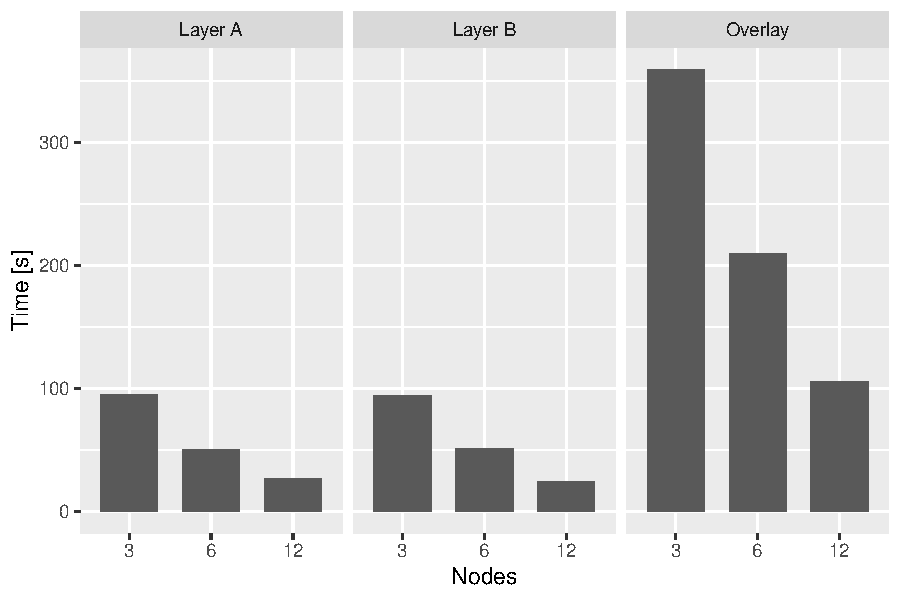
\includegraphics[width=0.49\linewidth]{US_speedup.pdf} & 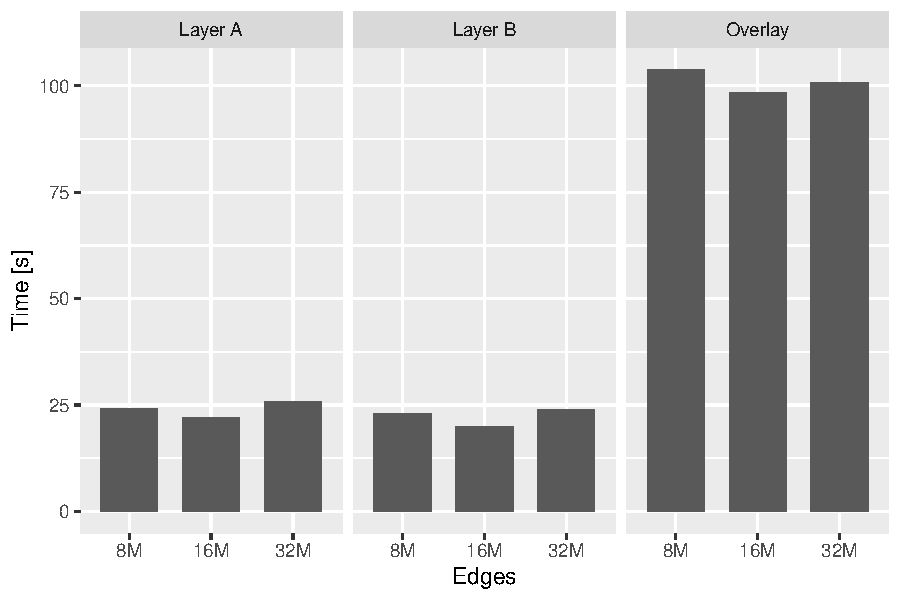
\includegraphics[width=0.49\linewidth]{US_scaleup.pdf} \\
        (a) & (b) 
    \end{tabular}
    \caption{(a)Speed Up and (b) Scale Up performance of the Kdtree partitioning using the MainUS dataset.} \label{fig:k_scale_speed_us}
\end{figure}



\subsection{Polygonization Scalability}
\label{sec:expr:query}


\begin{table}
    \caption{Polygonization Evaluation Dataset}
    \label{table:polygonization:datasets}
    \begin{tabular}{c c c c c}
        \toprule
        Dataset  & Area & Number of Line Segments & Faces \\
        \midrule
        USA & 9.83 $Mkm^2$ & 152$M$ & 5$M$ \\
        South America & 17.8 $Mkm^2$ & 155$M$ & 7$M$\\
        North America & 24.7 $Mkm^2$ & 240$M$ & 10$M$ \\
        Africa & 30.4 $Mkm^2$ & 288$M$ & 10$M$  \\
        Europe & 10.2 $Mkm^2$ & 563$M$ & 25$M$ \\ 
        Asia & 44.6 $Mkm^2$ & 557$M$ & 23$M$ \\ 
        \bottomrule
    \end{tabular}
\end{table}

\begin{figure}
\centering
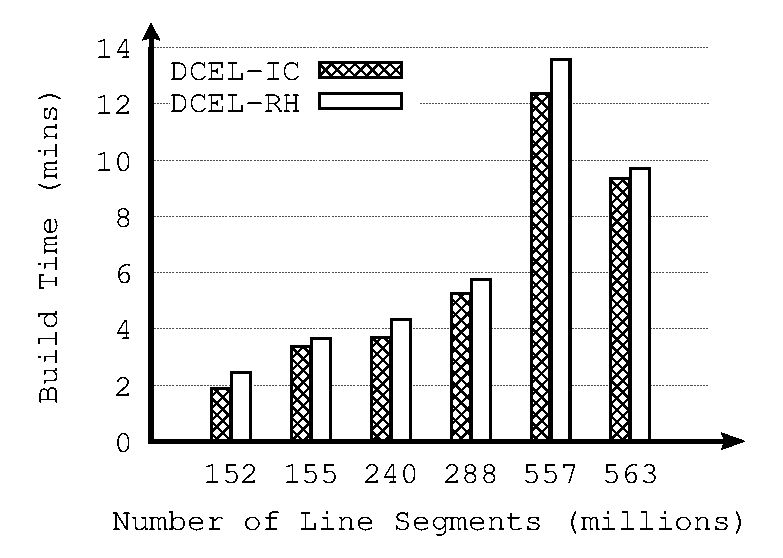
\includegraphics[width=0.48\linewidth]{Experiments/n_records.eps}
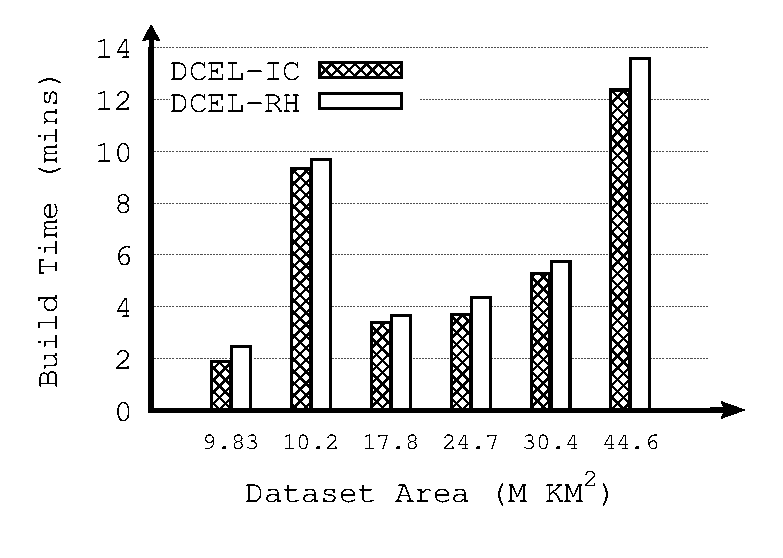
\includegraphics[width=0.48\linewidth]{Experiments/area.eps}
\caption{Polygonization Performance on Real Road Networks.}
\label{fig:exp:query}
\end{figure}

Figure~\ref{fig:exp:query} evaluates the scalability of the polygonization approach using the different evaluation datasets summarized in Table \ref{table:polygonization:datasets}. 
We implemented our polygonization framework on Apache Sedona \cite{YZS18}. The experiment is based on a Java 8 implementation and utilizes a Spark 2.3 cluster with two driver nodes and 12 worker nodes. All nodes run Linux CentOS 8.2 (64-bit). Each driver node is equipped with 128GB of RAM, while each worker node has 64GB of RAM. To increase parallelism, we divided the 12 worker nodes into 84 worker executors. Each executor is a separate JVM process with dedicated resources, such as memory and CPU cores. The distribution of these executors across the nodes is managed by the resource negotiator (YARN), which allocates resources for Spark jobs based on the availability of cores and memory. YARN typically balances resources across the cluster, so executors are likely to be evenly distributed, though some variation may occur due to resource availability at runtime. Assuming an even distribution, each worker node would run approximately 7 executors, as calculated by $\frac{84}{12} = 7$.

As discussed in Section~\ref{sec:rem}, the Rem Phase has two different approaches depending on the input data received from the Gen Phase. The first approach is to process the remaining half-edges iteratively, denoted as \textit{DCEL-RH}. In comparison, the second approach processes the incomplete cycles generated from the first phase iteratively denoted as \textit{DCEL-IC}.

From Figure~\ref{fig:exp:query}, we draw three conclusions; 
(1) first, the cardinality of the input dataset has a positive correlation with the build time; as the number of line segments increases, the build time also increases, as shown in Figure~\ref{fig:exp:query}(a). However, we see that we have close cardinality for Asia (557M) and Europe (563M) datasets, but there is a noticeable difference in the build time; moreover, the build time for the Europe dataset is less than that of the Asia dataset. 
This drives us to the second conclusion;  
(2)~for datasets with close or similar cardinalities, the area of the dataset has a positive correlation with the build time shown in Figure~\ref{fig:exp:query}(b). 
Hence the build time of the Europe dataset (10.2 $Mkm^2$) is less than that of the Asia dataset (44.6 $Mkm^2$), even though Europe has a slightly larger dataset.
(3)~The third conclusion is that for all evaluated datasets, the \textit{DCEL-IC} beats \textit{DCEL-RH}.

\subsection{Polygonization Speed Up Evaluation}
\label{sec:expr:speedup}

\begin{figure}[tb]
	\centering
	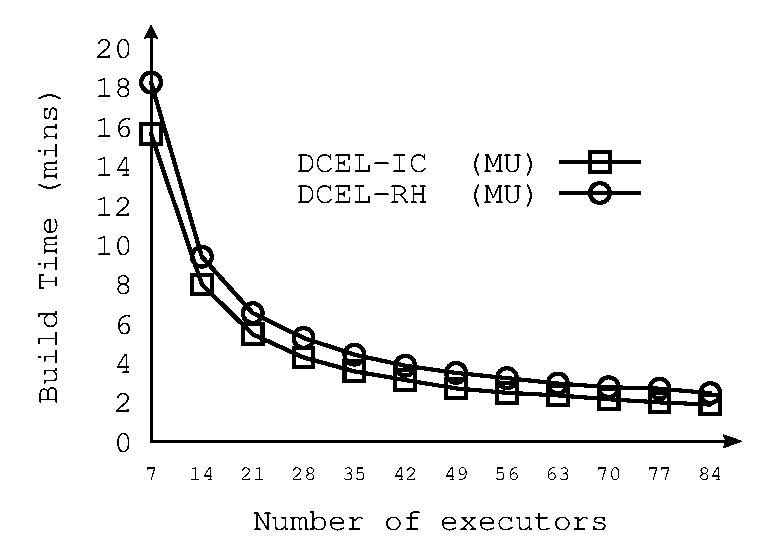
\includegraphics[width=8.8cm]{Experiments/speedup.eps}
	\caption[caption]{Polygonization speed up evaluation using the USA dataset}
	\label{fig:exp:speedup}
\end{figure}

Figure~\ref{fig:exp:speedup} shows the effect of increasing the number of executors on the build time for the USA dataset. 
At each step in the figure, we add 7 more executors, which is approximately equivalent to adding one additional node.
Overall, our approach has good speedup performance. As the number of executors is doubled from 7~executors to 14~executors, the build time is almost halved. This trend goes on as we double the number of executors. As we increase the number of executors from 7 to 84, the build time is decreased by a factor of 8. 

\subsection{Overlaying Polygons with Dangle and Cut Edges}

\begin{table}
    \caption{Overlaying Polygons with Dangle and Cut Edges Dataset}
    \label{tab:dangles}
    \begin{tabular}{c c c c}
        \toprule
        Dataset & Number Layer $A$ of Polygons & Number of Layer $B$ Edges & Result Polygons \\
        \midrule
        TN & 1,272 & 3,380,780 & 41,761 \\
        GA & 1,633 & 4,647,171 & 49,125 \\
        NC & 1,272 & 7,212,604 & 22,413 \\
        TX & 4,399  & 8,682,950 & 98,635 \\
        VA & 1,554 & 8,977,361 & 38,941 \\
        CA & 7,038 & 9,103,610 & 96,916\\
        \bottomrule
    \end{tabular}
\end{table}


\begin{figure}
    \centering
    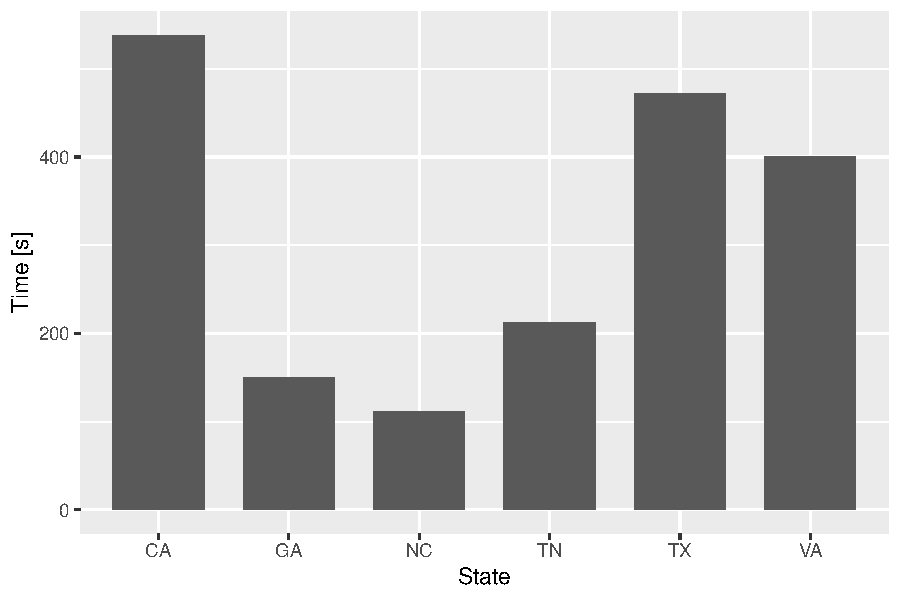
\includegraphics[width=0.7\linewidth]{states.pdf}
    \caption{Overlaying State polygons with dangle and cut edges.}
    \label{fig:dangle}
\end{figure}

In this section, we examine the performance of overlaying polygons with dangle and cut edges resulting from the polygonization as detailed in Section \ref{sec:over_dang}.
Table \ref{tab:dangles} shows the number of polygons for each state for the first layer of the overlay. It also shows the number of dangle and cut edges per state for the second layer of the overlay. Finally, it shows the number of resultant polygons per state.
From Figure \ref{fig:dangle}, we conclude that the running time is affected by the number of dangle and cut edges and the number of intersections between the two layers (represented by the number of generated polygons). 
TN and GA have a relatively smaller number of dangle and cut edges, so they have lower execution times compared to VA, TX, and CA. However, since the intersections in NC are significantly less than those of TN and GA, NC has the lowest execution time. TX, VA, and CA have a comparable number of edges; however, VA has the least number of intersections, resulting in lower execution time compared to TX and CA. 


%%
%% If your work has an appendix, this is the place to put it.
%%
%%\appendix
%%\input{appendices}

%%
%% The next two lines define the bibliography style to be used, and the bibliography file.
%%
\bibliographystyle{ACM-Reference-Format}
\bibliography{sdcel}

\end{document}
